\documentclass[
  man,
  longtable,
  a4paper,
  nolmodern,
  notxfonts,
  notimes,
  colorlinks=true,linkcolor=blue,citecolor=blue,urlcolor=blue]{apa7}

\usepackage{amsmath}
\usepackage{amssymb}




\RequirePackage{longtable}
\RequirePackage{threeparttablex}

\makeatletter
\renewcommand{\paragraph}{\@startsection{paragraph}{4}{\parindent}%
	{0\baselineskip \@plus 0.2ex \@minus 0.2ex}%
	{-.5em}%
	{\normalfont\normalsize\bfseries\typesectitle}}

\renewcommand{\subparagraph}[1]{\@startsection{subparagraph}{5}{0.5em}%
	{0\baselineskip \@plus 0.2ex \@minus 0.2ex}%
	{-\z@\relax}%
	{\normalfont\normalsize\bfseries\itshape\hspace{\parindent}{#1}\textit{\addperi}}{\relax}}
\makeatother




\usepackage{longtable, booktabs, multirow, multicol, colortbl, hhline, caption, array, float, xpatch}
\usepackage{subcaption}


\renewcommand\thesubfigure{\Alph{subfigure}}
\setcounter{topnumber}{2}
\setcounter{bottomnumber}{2}
\setcounter{totalnumber}{4}
\renewcommand{\topfraction}{0.85}
\renewcommand{\bottomfraction}{0.85}
\renewcommand{\textfraction}{0.15}
\renewcommand{\floatpagefraction}{0.7}

\usepackage{tcolorbox}
\tcbuselibrary{listings,theorems, breakable, skins}
\usepackage{fontawesome5}

\definecolor{quarto-callout-color}{HTML}{909090}
\definecolor{quarto-callout-note-color}{HTML}{0758E5}
\definecolor{quarto-callout-important-color}{HTML}{CC1914}
\definecolor{quarto-callout-warning-color}{HTML}{EB9113}
\definecolor{quarto-callout-tip-color}{HTML}{00A047}
\definecolor{quarto-callout-caution-color}{HTML}{FC5300}
\definecolor{quarto-callout-color-frame}{HTML}{ACACAC}
\definecolor{quarto-callout-note-color-frame}{HTML}{4582EC}
\definecolor{quarto-callout-important-color-frame}{HTML}{D9534F}
\definecolor{quarto-callout-warning-color-frame}{HTML}{F0AD4E}
\definecolor{quarto-callout-tip-color-frame}{HTML}{02B875}
\definecolor{quarto-callout-caution-color-frame}{HTML}{FD7E14}

%\newlength\Oldarrayrulewidth
%\newlength\Oldtabcolsep


\usepackage{hyperref}




\providecommand{\tightlist}{%
  \setlength{\itemsep}{0pt}\setlength{\parskip}{0pt}}
\usepackage{longtable,booktabs,array}
\usepackage{calc} % for calculating minipage widths
% Correct order of tables after \paragraph or \subparagraph
\usepackage{etoolbox}
\makeatletter
\patchcmd\longtable{\par}{\if@noskipsec\mbox{}\fi\par}{}{}
\makeatother
% Allow footnotes in longtable head/foot
\IfFileExists{footnotehyper.sty}{\usepackage{footnotehyper}}{\usepackage{footnote}}
\makesavenoteenv{longtable}

\usepackage{graphicx}
\makeatletter
\newsavebox\pandoc@box
\newcommand*\pandocbounded[1]{% scales image to fit in text height/width
  \sbox\pandoc@box{#1}%
  \Gscale@div\@tempa{\textheight}{\dimexpr\ht\pandoc@box+\dp\pandoc@box\relax}%
  \Gscale@div\@tempb{\linewidth}{\wd\pandoc@box}%
  \ifdim\@tempb\p@<\@tempa\p@\let\@tempa\@tempb\fi% select the smaller of both
  \ifdim\@tempa\p@<\p@\scalebox{\@tempa}{\usebox\pandoc@box}%
  \else\usebox{\pandoc@box}%
  \fi%
}
% Set default figure placement to htbp
\def\fps@figure{htbp}
\makeatother


% definitions for citeproc citations
\NewDocumentCommand\citeproctext{}{}
\NewDocumentCommand\citeproc{mm}{%
  \begingroup\def\citeproctext{#2}\cite{#1}\endgroup}
\makeatletter
 % allow citations to break across lines
 \let\@cite@ofmt\@firstofone
 % avoid brackets around text for \cite:
 \def\@biblabel#1{}
 \def\@cite#1#2{{#1\if@tempswa , #2\fi}}
\makeatother
\newlength{\cslhangindent}
\setlength{\cslhangindent}{1.5em}
\newlength{\csllabelwidth}
\setlength{\csllabelwidth}{3em}
\newenvironment{CSLReferences}[2] % #1 hanging-indent, #2 entry-spacing
 {\begin{list}{}{%
  \setlength{\itemindent}{0pt}
  \setlength{\leftmargin}{0pt}
  \setlength{\parsep}{0pt}
  % turn on hanging indent if param 1 is 1
  \ifodd #1
   \setlength{\leftmargin}{\cslhangindent}
   \setlength{\itemindent}{-1\cslhangindent}
  \fi
  % set entry spacing
  \setlength{\itemsep}{#2\baselineskip}}}
 {\end{list}}
\usepackage{calc}
\newcommand{\CSLBlock}[1]{\hfill\break\parbox[t]{\linewidth}{\strut\ignorespaces#1\strut}}
\newcommand{\CSLLeftMargin}[1]{\parbox[t]{\csllabelwidth}{\strut#1\strut}}
\newcommand{\CSLRightInline}[1]{\parbox[t]{\linewidth - \csllabelwidth}{\strut#1\strut}}
\newcommand{\CSLIndent}[1]{\hspace{\cslhangindent}#1}


\usepackage[nolongtablepatch]{lineno}
\linenumbers



\usepackage{newtx}

\defaultfontfeatures{Scale=MatchLowercase}
\defaultfontfeatures[\rmfamily]{Ligatures=TeX,Scale=1}





\title{Pre-registered report: Mapping Synesthetic Sequences in Space:
Improving Consistency Test by Harnessing Cartography Tools.}


\shorttitle{Space-Sequence Synesthesia: Optimizing Consistency Tests}


\usepackage{etoolbox}








\authorsnames{Rémy Lachelin,Chhavi Sachdeva,Nicolas Rothen}





\affiliation{
{Psychology, UniDistance Suisse}}




\leftheader{Lachelin, Sachdeva and Rothen}



\abstract{Sequence-space synesthesia is a perceptual condition in which
ordinal sequences (e.g., numbers, days of the week, or months of the
year) are experienced as occupying specific spatial locations. This
perceptual condition is identified using self-reports
(e.g.~questionnaires) and behavioural consistency tasks. Existing
consistency tests measure the spatial distance between responses to
repeated stimuli, but they ignore the ordinal and geometric features of
spatial-forms. This preregistered study consists of a present and future
analyses. In the present analyses, we optimise SSS diagnostics from
consistency test by extracting novel geometric features at the
spatial-form level. To do this, we first evaluate classification
performances of old and new features in a large (N = 685) aggregated
sample from four available and independent datasets. We then harness a
geographic toolbox to extract metrics from the spatial-forms level.
Finally, receiver operating characteristic (ROC) analyses are conducted
to assess the discriminative performances of each method. The results
show that permuted topological validity of spatial-forms and the
perimeter between stimuli performs equally well in detecting SSS. In a
future study, we will examine predictive validity of the selected
methods on an independent dataset that has yet to be collected. Findings
from the present study highlight the relevance of topological principles
for sequence-space representations and aims to optimise the ability of
consistency tests to detect SSS. }

\keywords{Sequence space
synaesthesia, Synaesthesia/synesthesia, consistency
test, space, time, numbers}

\authornote{\par{\addORCIDlink{Rémy
Lachelin}{0000-0002-8485-7153}}\par{\addORCIDlink{Chhavi
Sachdeva}{0000-0002-0074-4371}}\par{\addORCIDlink{Nicolas
Rothen}{0000-0002-8874-8341}} 

\par{       Author roles were classified using the Contributor Role
Taxonomy (CRediT; https://credit.niso.org/) as follows:  Rémy
Lachelin:   Conceptualization, Methodology, Formal Analysis, Data
Curation, Writing - Original Draft; Chhavi
Sachdeva:   Conceptualization, Methodology, Writing - Review \&
Editing; Nicolas Rothen:   Conceptualization, Writing - Review \&
Editing, Supervision, Project Administration, Founding Acquisition}
\par{Correspondence concerning this article should be addressed to Rémy
Lachelin, Psychology, UniDistance Suisse, Schinerstrasse
18, Brig-Glis, Valais 3900, Email: \href{mailto:remy.lachelin@fernuni.ch}{remy.lachelin@fernuni.ch}}
}

\makeatletter
\let\endoldlt\endlongtable
\def\endlongtable{
\hline
\endoldlt
}
\makeatother
\RequirePackage{longtable}
\DeclareDelayedFloatFlavor{longtable}{table}

\urlstyle{same}



\makeatletter
\@ifpackageloaded{caption}{}{\usepackage{caption}}
\AtBeginDocument{%
\ifdefined\contentsname
  \renewcommand*\contentsname{Table of contents}
\else
  \newcommand\contentsname{Table of contents}
\fi
\ifdefined\listfigurename
  \renewcommand*\listfigurename{List of Figures}
\else
  \newcommand\listfigurename{List of Figures}
\fi
\ifdefined\listtablename
  \renewcommand*\listtablename{List of Tables}
\else
  \newcommand\listtablename{List of Tables}
\fi
\ifdefined\figurename
  \renewcommand*\figurename{Figure}
\else
  \newcommand\figurename{Figure}
\fi
\ifdefined\tablename
  \renewcommand*\tablename{Table}
\else
  \newcommand\tablename{Table}
\fi
}
\@ifpackageloaded{float}{}{\usepackage{float}}
\floatstyle{ruled}
\@ifundefined{c@chapter}{\newfloat{codelisting}{h}{lop}}{\newfloat{codelisting}{h}{lop}[chapter]}
\floatname{codelisting}{Listing}
\newcommand*\listoflistings{\listof{codelisting}{List of Listings}}
\makeatother
\makeatletter
\makeatother
\makeatletter
\@ifpackageloaded{caption}{}{\usepackage{caption}}
\@ifpackageloaded{subcaption}{}{\usepackage{subcaption}}
\makeatother

% From https://tex.stackexchange.com/a/645996/211326
%%% apa7 doesn't want to add appendix section titles in the toc
%%% let's make it do it
\makeatletter
\xpatchcmd{\appendix}
  {\par}
  {\addcontentsline{toc}{section}{\@currentlabelname}\par}
  {}{}
\makeatother

%% Disable longtable counter
%% https://tex.stackexchange.com/a/248395/211326

\usepackage{etoolbox}

\makeatletter
\patchcmd{\LT@caption}
  {\bgroup}
  {\bgroup\global\LTpatch@captiontrue}
  {}{}
\patchcmd{\longtable}
  {\par}
  {\par\global\LTpatch@captionfalse}
  {}{}
\apptocmd{\endlongtable}
  {\ifLTpatch@caption\else\addtocounter{table}{-1}\fi}
  {}{}
\newif\ifLTpatch@caption
\makeatother

\begin{document}

\maketitle



\setcounter{secnumdepth}{3}

\setlength\LTleft{0pt}

\resetlinenumber[1]



\section{Introduction}\label{sec-introduction}
Test add things here
Sequence-Space Synaesthesia (SSS) or visuo-spatial forms is the
phenomenon where people visualize ordered sequences in particular
spatial positions. bers, weekdays or months (synesthetic
\emph{inducers}) are represented as arranged into specific spatial
positions in space (synesthetic \emph{concurrent}). The synaesthetic
spatial-forms can be complex and have variable geometric forms. Those
geometric forms might be different for each categories
(i.e.~number-forms weekdays and months), with forms such as ellipses,
zig-zags or curbed lines Flournoy (\citeproc{ref-flournoy1893}{1893}).
SSS are usually identified using questionnaires and consistency tests.
An individual is identified as SSS based on the variability at the
stimulus level between repeated responses: less variable responses being
an indicator of the consistent response characteristic of SSS. However,
stimulus level consistency can also be achieved by responding to the
same position for all stimuli. Furthermore, it might favour linear over
circular spatial-forms and is not informed about the ordinality between
stimuli (e.g.~1 \texttt{→} 2 \texttt{→} 3, etc.). Here, we aim at
optimizing the identification of SSS from consistency tasks using
geometrical characteristics of spatial-forms from ordered stimuli or
inducers.

SSS frequently co-occurs with other subtypes of synaesthesia and as for
other subtypes of synaesthesia it's idiosyncratic. Colour-grapheme
synaesthesia, where a grapheme \emph{inducer} triggers a
\emph{concurrent} colour (i.e.~``A'' seen as red), co-occurs at 71 \% to
76 \% with SSS (\citeproc{ref-sagiv2006}{Sagiv et al., 2006}).
Nevertheless, across different synaesthetic subtypes, self-reported SSS
tend to cluster together (\citeproc{ref-ward2022}{Ward \& Simner,
2022}), indicating a degree of internal homogeneity and justifying to
study it as a distinct phenomenon. Spatial-forms are idiosyncratic,
which results in considerable heterogeneity in how this phenomenon is
manifested across individuals. One source of heterogeneity is given by
dimensionality: some SSS experiences can involve three-dimensional (3D)
and two-dimensional (2D) arrangements
(\citeproc{ref-eagleman2009a}{Eagleman, 2009};
\citeproc{ref-price2013}{Price \& Pearson, 2013}). Another source of
heterogeneity is the reference frame, for example, the spatial-forms
might take place in an external space around the body (\emph{i.e.}
projector) or in an egocentric internal space (\emph{i.e.} associator)
(\citeproc{ref-dixon2004}{Dixon et al., 2004};
\citeproc{ref-smilek2007}{Smilek et al., 2007}). Further variability can
be explained by temporal-spatial properties and mental-manipulation of
spatial-forms such as ``zooming'' in and out or rotating or shifting
perspectives at will (\citeproc{ref-gould2014}{Gould et al., 2014};
\citeproc{ref-jarick2009}{Jarick et al., 2009}) Lastly, the shape,
complexity and layout of the spatial-forms are also heterogeneous such
as forming for example ovals, lines, zig-zags or loops. With some
recurring shapes being more frequent across SSS, such as ovals for
months (\citeproc{ref-eagleman2009a}{Eagleman, 2009}).

Despite the after mentioned heterogeneities, SSS is also
phenomenological characterized. There might be five main characteristics
for synaesthesia in general and specifically SSS
(\citeproc{ref-deroy2013}{Deroy \& Spence, 2013};
\citeproc{ref-seron1992}{Seron et al., 1992}). \emph{Automaticity}: the
inducer automatically triggers the concurrent. \emph{Unidirectionality}:
while the \emph{inducer} triggers the concurrent, the concurrent does
not trigger the inducer. \emph{Developmentally}: the experience was
already present during childhood. \emph{Consciousness}: The concurrent
is consciously perceived. \emph{Consistency}: the inducer-concurrent
pair remains stable in time within subject. While some of these
characteristics can be captured with self-reported questionnaire
(i.e.~for development and consciousness), other can be quantified more
objectively using behavioural tasks such as consistency tests
(\citeproc{ref-baron-cohen1993}{Baron-Cohen et al., 1993}).

\subsection{Consistency tests}\label{sec-consistency-tests}

Consistency tests are extracted form behavioural tasks used to evaluate
how stable synesthetic experiences are over time
(\citeproc{ref-rothen2013a}{Rothen et al., 2013},
\citeproc{ref-rothen2016}{2016}). They do this by presenting the same
stimuli repeatedly and assessing how similar participant's responses are
across repetitions (i.e.~\emph{inducer}-\emph{concurrent} associations).
High consistency is often taken as evidence for synaesthesia.
Consistency tests have proven effective for colour-grapheme
synaesthesia. Measures of individual consistency can be derived using
colour pickers while repeatedly presenting the same inducer
(i.e.~``A''). The quantification of the distance between concurrents
from the same inducers is used to discriminate consistent synaesthetes
from controls. Specifically, the euclidean distance in CIE L*u*v colour
space, which is designed for perceptual uniformity, yields optimal
classification accuracy when using a cut-off estimated as deduced from a
larger representative sample (\citeproc{ref-rothen2013a}{Rothen et al.,
2013}). A similar rationale to that used for colour-grapheme
synaesthesia has been applied to characterize SSS from consistency
tasks.

In the SSS consistency task, participants complete multiple rounds of
the same stimuli (e.g., digits, days of the week, and months of the
year) and are asked to indicate a spatial location for each stimulus by
clicking on the computer screen. Brang et al.
(\citeproc{ref-brang2010}{2010}) for example evaluated consistency as
the distance between repeated responses to the same inducer or stimuli
(e.g.~January and January) relative to adjacent stimuli (e.g.~February).
A response was defined as consistent if it fell within 1.96
\emph{z-scores}. However, this criterion was noted to be potentially too
conservatory, as it identified synaesthesia in 4 of 81 self-reported
synaesthetes. Geometrical features such as area and perimeter between
the coordinates of repeated inducers have further been used as a measure
of the distance between same inducers, hence as a metric for
consistency. Less consistent responses leading to smaller triangle
perimeters and area (\citeproc{ref-rothen2016}{Rothen et al., 2016}). A
cut-off corresponding to less than 0.203 \% average responses area in
proportion to the total screen area to classify as SSS has been
suggested (see also \citeproc{ref-ward2018}{Ward et al., 2018}).

However, several general caveats of consistency tests using concurrent
or stimulus level metrics have been identified. Some tests may favour
certain spatial-forms (\citeproc{ref-ward2018}{Ward et al., 2018}) in
particular those with linear or highly regular spatial layouts,
i.e.~elliptical patterns for months(\citeproc{ref-brang2010}{Brang et
al., 2010}; \citeproc{ref-eagleman2009a}{Eagleman, 2009};
\citeproc{ref-flournoy1893}{Flournoy, 1893}). Another concern is that
participants that respond with the same position, for example when not
knowing the response, will have artificially high consistencies with
those metrics (\citeproc{ref-rothen2016}{Rothen et al., 2016}). This has
led to alternative approaches such as to add the standard deviation of
responses, questionnaire cut-off (\citeproc{ref-ward2018}{Ward et al.,
2018}) or permutation-based comparison of individual responses to chance
levels for colour-grapheme (\citeproc{ref-root2021}{Root et al., 2021})
and SSS (\citeproc{ref-ward2022a}{Ward, 2022}). Finally, these
consistency tests evaluate the variability of responses to the same
stimuli, therefore the ordinality between stimuli is not taken into
account. Synaesthetic spatial-forms follow ordinal rules (e.g.~Monday
\texttt{→} Tuesday \texttt{→} Wednesday). In the domain of numerical
cognition, ordinality has been identified as an important information
when processing sequences (\citeproc{ref-lyons2013}{Lyons \& Beilock,
2013}). Some studies of SSS have systematically investigated ordinality
by investigating metrics of adjacent inducer-concurrent pairs such as
distances (\citeproc{ref-brang2010}{Brang et al., 2010}) or angles
(\citeproc{ref-eagleman2009a}{Eagleman, 2009}). However, ordinality of
the concurrent spatial-form might be particularly relevant considering
all the stimuli of a certain category (i.e.~weekdays or months). The
spatial-forms of the concurrents are often spatially structured into
configuration such as lines or polygons that may follow distinctive
geometrical rules. For example linear layouts have been described in
early accounts of number forms (\citeproc{ref-flournoy1893}{Flournoy,
1893}; \citeproc{ref-galton1880}{Galton, 1880}).

\subsection{Present study}\label{present-study}

The goal of this registered report is to compare different consistency
tests on their classification performances of individuals with SSS and
controls doing the consistency task using Receiver Operator
Characteristics (ROC) analyses. In the present \emph{Phase I}, we merge
four previously available datasets using the same task on both SSS and
control groups (\citeproc{ref-ward2022a}{Ward, 2022}). First, we aimed
to reproduce established consistency test methods based on
stimulus-level consistency metrics, such as area and perimeter. Second,
we explored a new approach comparing geometrical features across
repetitions of the same categories (weekday, month and numbers), such as
segments and polygons. These novel tests are designed to take advantage
of the sequentiality or ordinality between the responses and the
geometrical properties at the spatial-form level, see
Figure~\ref{fig-myplot00}. All the consistency tests are then compared
using ROC analyses on their correct classification performances of
self-reported SSS and control groups.

In a future study, we will assess whether the tests identified in the
present study generalize and are validated on an independent dataset
that is yet to be acquired (Sachdeva et al.
(\citeproc{ref-sachdeva2024}{2024}), Stage 1 in-principle acceptance,
see also \url{https://osf.io/6wn4m}).

\section{Methods}\label{methods}

Code and data for ``one-click'' reproducibility of this manuscript
including the following analyses are available on git-hub
(\url{https://github.com/remLach/SpaceSequenceSynDiagnostic}). All the
analyses are conducted in R, using the following packages `pROC' v.
1.19.0.1 (\citeproc{ref-pROC}{Robin et al., 2011}), `sf' v. 1.0.21
(\citeproc{ref-sf}{Pebesma \& Bivand, 2023}) and for visualization
`ggplot2' v. 4.0.1 (\citeproc{ref-ggplot2}{Wickham, 2016}),
`ggVennDiagram' v. 1.5.6 (\citeproc{ref-ggVennDiagram}{Gao \& Dusa,
2025}).

\subsection{\texorpdfstring{\emph{Datasets and
Participants}}{Datasets and Participants}}\label{datasets-and-participants}

To base the optimization of the consistency test on the largest possible
sample we looked for accessible datasets that used the same consistency
tasks on groups of synesthetes and controls. We found four datasets that
met these criteria. Two datasets were collected in laboratory settings
Rothen et al. (\citeproc{ref-rothen2016}{2016}) (see also
\href{https://osf.io/6hq94/files/osfstorage}{https://osf.io/6hq94}) and
Van Petersen et al. (\citeproc{ref-vanpetersen2020}{2020}) (see also
\url{https://data.ru.nl/collections/di/dcc/DSC_2018.00019_653}). The two
others came from on-line testing Ward (\citeproc{ref-ward2022a}{2022})
(see also\url{https://osf.io/nu5v4}) and an additional dataset was
gently provided by private communications with Professor Ward. To match
the other datasets, stimuli of the weekdays and months categories were
translated from Dutch to English in the dataset from
(\citeproc{ref-vanpetersen2020}{Van Petersen et al., 2020}). For the
number category we included only digits from 0 to 9 that where presented
across all datasets (i.e.~excluding the stimuli ``50'' and ``100'' for
numbers in Van Petersen et al. (\citeproc{ref-vanpetersen2020}{2020})).

From the merged datasets, we kept 685 from the total 689 participants.
First, we excluded 0.02 \% empty trials (i.e.~skipped responses)
including trials flagged for having the same x or y coordinates across
conditions and repetitions, causing the depletion n = 2 participants(as
in \citeproc{ref-rothen2016}{Rothen et al., 2016};
\citeproc{ref-ward2018}{Ward et al., 2018}). n = 2 participants were
excluded for having less than 4 coordinate points since polygons need at
least four coordinate. Note therefore, that 31 participants of the final
sample did not have responses in all three conditions X repetition
cases. From the final sample of N = 685, 396 were synaesthetes and 289
controls, see Table~\ref{tbl-mytable01} and Table~\ref{tbl-mytable02}.

\begin{table}

{\caption{{Synesthetes}{\label{tbl-mytable01}}}
\vspace{-20pt}}

\begin{longtable}[]{@{}llll@{}}
\toprule\noalign{}
Synaesthetes & N before & N after & Age \\
\midrule\noalign{}
\endhead
\bottomrule\noalign{}
\endlastfoot
(\citeproc{ref-rothen2016}{Rothen et al., 2016}) & 33 & 32 & 23.1 \\
(\citeproc{ref-vanpetersen2020}{Van Petersen et al., 2020}) & 23 & 22 &
23.2 \\
(\citeproc{ref-ward2022a}{Ward, 2022}) & 252 & 252 & 37.2 \\
Ward 2 & 90 & 90 & NA \\
Total: & 398 & 396 & \\
\end{longtable}

\vspace{-20pt}
\noindent \emph{Note.} Synesthetes.~Demographics were not provided in
the dataset Ward 2. Before: before participant exclusion

\end{table}

\begin{table}

{\caption{{Controls}{\label{tbl-mytable02}}}
\vspace{-20pt}}

\begin{longtable}[]{@{}llll@{}}
\toprule\noalign{}
Controls & N before & N after & Age \\
\midrule\noalign{}
\endhead
\bottomrule\noalign{}
\endlastfoot
(\citeproc{ref-rothen2016}{Rothen et al., 2016}) & 37 & 37 & 28.2 \\
(\citeproc{ref-vanpetersen2020}{Van Petersen et al., 2020}) & 21 & 21 &
21.6 \\
(\citeproc{ref-ward2022a}{Ward, 2022}) & 215 & 213 & 19.9 \\
Ward 2 & 18 & 18 & NA \\
Total & 291 & 289 & \\
\end{longtable}

\vspace{-20pt}
\noindent \emph{Note.} Controls.~Demographics were not provided in the
dataset Ward 2. Before: before participant exclusion

\end{table}

Regarding the synaesthets profiles, detailed participant information
such as questionnaire responses were only available from the two
datasets from the data by Professor Ward (i.e.~a majority of 573
participants). We described the self-reported profiles for the stimulus
categories used in the consistency test (i.e.~number, weekdays and
month), see Figure~\ref{fig-myplot01}. From this Venn-diagram we see
that 240 of the SSS report having spatial-forms for Numbers, Days and
Month; 42 only Days and Month; 21 only Number and Day. Also, 127
controls report spatial-forms for either Days, Numbers, Months or
combinations.

\begin{figure}[!htbp]

{\caption{{Venn diagram of the types of self-reported
SSS}{\label{fig-myplot01}}}}

\pandocbounded{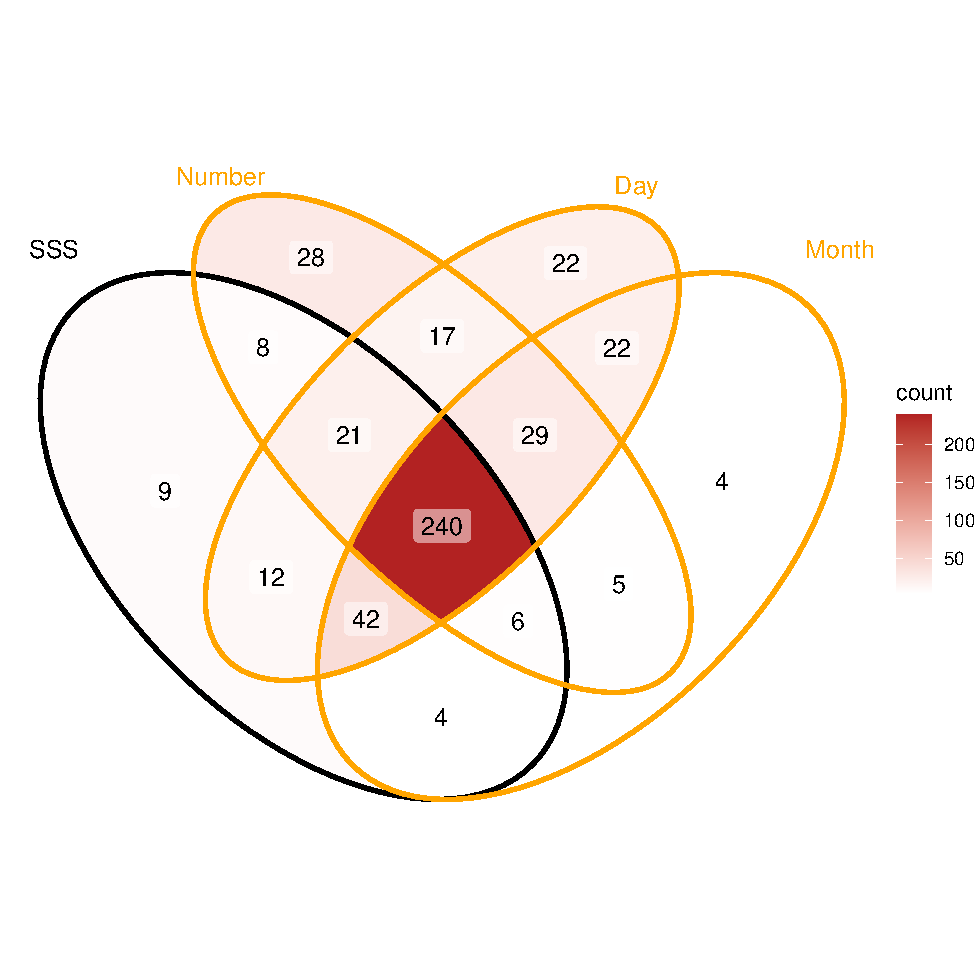
\includegraphics[keepaspectratio]{2.RegisteredReport_MS2_files/figure-pdf/fig-myplot01-1.pdf}}

\vspace{-20pt}
\noindent \emph{Note.} Only~data from Pr. Ward is represented here. SSS
= Sequence-space synaesthesia

\end{figure}

\subsection{Procedure}\label{procedure}

For the consistency task, each stimuli were presented randomly and
sequentially centrally on the screen. Participant were instructed to
click on the screen position where they visualize them. In Van Petersen
et al. (\citeproc{ref-vanpetersen2020}{2020}) and Rothen et al.
(\citeproc{ref-rothen2016}{2016}) the participants were allowed to skip
responses.

Stimulus included here were 7 weekdays (Monday to Sunday), 12 months
(January to December) and 9 numbers (0 to 9). For all the data from
Professor Ward the stimuli were presented in randomized order with the
constraint that no stimulus was repeated until all unique stimuli (N =
29) had been presented once. The median display resolution was 1440 X
768, with a maximum of 2560 X 2025 and a minimum of 308 X 149.

\subsection{Analyses}\label{analyses}

\subsubsection{\texorpdfstring{Consistency tests on the \emph{stimulus
level}}{Consistency tests on the stimulus level}}\label{consistency-tests-on-the-stimulus-level}

We reproduced the tests extracted from consistency tasks found in the
literature such as area and perimeter between repetitions
(\citeproc{ref-rothen2016}{Rothen et al., 2016};
\citeproc{ref-vanpetersen2020}{Van Petersen et al., 2020};
\citeproc{ref-ward2022a}{Ward, 2022}). Formally, the area (see
Equation~\ref{eq-area}) and perimeter (see Equation~\ref{eq-perim}) are
calculated from the triangle (i.e.~given three repetitions) formed by
the \emph{x} and \emph{y} coordinates of the three repetitions of each
stimuli (i.e.~\emph{(x1, y1), (x2, y2), (x3, y3)}).

\begin{equation}\phantomsection\label{eq-area}{
Area = \frac{|x1y2 +x2y3 + x3y1 – x1y3 – x2y1 – x3y2|}{2}
}\end{equation}

\begin{equation}\phantomsection\label{eq-perim}{
Perimeter = \sqrt{(x2 - x1)^2 + (y2 – y1)^2} + \sqrt{(x3 - x2)^2 + (y3 –y2)^2} + \sqrt{(x1 - x3)^2 + (y1 – y3)^2}
}\end{equation}

Each stimuli's area was then averaged by participants. The area metric
is in \% of the screen area to be able to compare with the consistency
across studies using different screen sizes. To account for screen size
and spread variability across the datasets and participants, area and
perimeter were also calculated on individually normalized x and y
coordinates (\emph{z-score}). These methods compute consistency metrics
at the stimulus level, the rationale is that consistent responses would
show less variability between repetitions. For example, smaller area or
perimeter of the triangle formed indicate more variability hence more
consistent responses between the three repetitions.

\subsubsection{\texorpdfstring{Consistency tests on the \emph{space-form
level}}{Consistency tests on the space-form level}}\label{consistency-tests-on-the-space-form-level}

For the novel consistency tests, we extracted geometrical features at
the spatial-form level for each repetition separately. Taking the
stimuli as an ordered sequence we can consider them as a geometrical
segments (i.e.~open geometrical form) and polygons (i.e.~closed
geometrical form), similarly as originally described in Galton
(\citeproc{ref-galton1880}{1880}).

We harnessed a geospatial analysis, the `sf' package version 1.0.21
(\citeproc{ref-sf}{Pebesma \& Bivand, 2023}) to extract polyons and
geometry-based features from participant's 2D (x,y) coordinate
responses. This package allows, for example, to build and analyse
segments or polygons and then extract multiple geometrical descriptors
or features. Informed by the ordinality of the stimulus, we defined
segments and polygon by conditions and repetitions. The rationale here
was to determine whether, when considering the spatial-forms formed by
stimuli as ordered coordinates (i.e.~as segments or polygon) they remain
consistent \emph{between} repetitions for each individuals. We extracted
the topological validity, topological simplicity and a compactness score
for each polygons (i.e.~3 conditions X 3 repetitions: 9 polygons per
participants.

\paragraph{Segment
self-intersections.}\label{segment-self-intersections}

The first consistency test extracted from the segments is
self-intersection. We considered the spatial-forms as a segment
constituted by the lines connecting consecutive stimuli separately for
each category and repetitions (i.e.~Monday (repetition 1) \texttt{→}
Tuesday (repetition 1) \texttt{→} Wednesday (repetition 1), ect) and
then counted the number of times each segment self-intersect. The
rationale is that SSS should have less chance to produce that
self-intersect than control. The number of self-intersections were
computed separately for each repetitions and conditions and averaged per
participants.

\paragraph{Topological validity and
simplicity.}\label{topological-validity-and-simplicity}

We assessed topological validity using geometric validation test.
Topological validity tests if a polygons is well-formed and valid
according to the Open Geospatial Consortium (OGC) Simple Features
Specification (\citeproc{ref-herring2010}{Herring, 2010}). A polygon is
considered topologically valid if it satisfies the following criteria:
(1) if polygon rings are simple (i.e., they do not touch or
self-intersect), (2) boundary rings to not cross (3) boundary rings may
only touch points tangentially (4) rings that define holes are contained
within the exterior ring (5) the polygon rings must not splits the
polygon (\citeproc{ref-postgis}{\emph{PostGIS 3.6.2dev Manual}, n.d.}).
Topological simplicity evaluates whether a geometric object has a simple
structure without self-intersections or self-tangencies. According to
the OGC Simple Features Specification
(\citeproc{ref-herring2010}{Herring, 2010}), a polygon boundary is
considered simple if it does not pass through the same point more than
once (\citeproc{ref-postgis}{\emph{PostGIS 3.6.2dev Manual}, n.d.}). For
polygons, simplicity requires that each ring does not self-intersect or
self-touch. Note that simplicity is a condition for validity: a polygon
can be simple but still invalid (e.g., if an interior ring extends
outside the exterior ring).

For each participant we tested for topological validity and simplicity
across individual 3 categories (weekdays, month and numbers) and 3
repetitions, hence 9 space-forms or polygons. The binary outcome (1 = is
valid, 0 = invalid) was then averaged across all 9 forms. Hence, it can
span from 1 (all 9 are valid/simple) to 0 (none of the 9 forms are
valid/simple). Thus, the topological validity and simplicity score
ranges from 0 (none of the nine polygons are valid/simple) to 1 (all
nine polygons are valid). For example, if a participant's polygon for
weekdays were valid across all three repetitions, months were valid in
two of three repetitions, and numbers were invalid in all repetitions,
the topological validity score would be 5/9 ≈ 0.56.

\paragraph{Compactness score.}\label{compactness-score}

We also implemented a measure of compactness for the polygons. We used
the score developed to quantify the gerrymandering of political district
by Polsby and Popper (\citeproc{ref-polsby1991}{1991}). Gerrymandering
is a politically motivated strategy of redefining district's boundary to
give the advantage to a political party. This has the consequences to
reduce the compactness of those districts as would be expected if they
where defined from geomorphology. The compactness is calculated as the
ratio of the area and perimeter of a polygon. The rationale is that more
compact forms (i.e.~higher Polsby--Popper scores) would be more likely
in SSS than controls. Formally, the Polsby--Popper score is calculated
from the polygon's area and perimeter Equation~\ref{eq-PP}:

\begin{equation}\phantomsection\label{eq-PP}{
score = \frac{4\pi \cdot Area}{Perimeter^2}
}\end{equation}

\paragraph{Permutation-based feature
extraction.}\label{permutation-based-feature-extraction}

Finally, we implemented permutations of the repetition order to derive a
permuted measure of consistency. Specifically, instead of using
repetitions in chronological order, we shuffled the repetition order
between stimulus presentation (i.e.~Monday (repetition 2) \texttt{→}
Tuesday (repetition 3) \texttt{→} Wednesday (repetition 1), ect) and
extracted the geometrical feature from x,y coordinates of same stimulus
categories in non-chronological order The form-based tests computed
before were relying on the chronologically ordered repetitions. For
example, when a stimulus such as Monday was repeated three times, the
coordinates for the first presentation of Monday were always paired with
the coordinates for the first presentation of Tuesday to construct
segments or polygons. However, if synesthetic forms are truly
consistent, they should remain stable independently of the chronological
order of stimulus presentation. Hence, we permute the repetitions within
each condition. Specifically, for each participant and each category, we
randomized the response repetition order. For example segments for
weekdays were constructed with the x,y coordinates where randomly
permuted across repetition order, for example Monday (repetition 1),
Tuesday (repetition 3), Wednesday (repetition 2), ect. We predicted that
this permuted-based consistency would yield to better classification
performance (higher AUC values) compared to chronologically ordered
features. The rationale is that genuine synaesthetes would have a
consistently valid topology of spatial-forms repetitions regardless of
presentation order, whereas controls would show random variation. The
permutation scores were calculated for topological validity and
Polsby--Popper score.

\subsubsection{Receiver Operator Characteristic
analyses}\label{receiver-operator-characteristic-analyses}

Each of the previous method's performance in classifying SSS from
controls was compared with Receiver Operator Characteristics (ROC)
analyses. Classification performance was quantified using the area under
the curve (AUC), with higher AUC values indicating better discrimination
between SSS and control groups. The optimal cutoffs were calculated
using Youden's index(\citeproc{ref-youden1950}{Youden, 1950}).
Discriminant Power (DP) was used as an additional estimate of
discrimination performance according to the optimal cutoff
(Equation~\ref{eq-DP}). DP around 1 being interpreted as inefficient
discrimination.

\begin{equation}\phantomsection\label{eq-DP}{ 
DP = \frac{\sqrt{3}}{\pi} (\log(\frac{sensitivity}{1−sensitivity}) + \log(\frac{specificity}{(1−specificity)}))  
}\end{equation}

The statistical comparison of ROC curves between the methods was
operated testing the difference of AUC between pairs of curves using
bootstrapping method (1000 times) since it allows to compare methods
with different directions. Each bootstrap results in the subtraction of
the AUC between the two ROC. Then the each of the AUC difference's (D)
are divided by the standard deviation of those difference and compared
to a normal distribution (Equation~\ref{eq-D}).

\begin{equation}\phantomsection\label{eq-D}{
D = \frac{AUC_1-AUC_2}{SD}
}\end{equation}

Therefore we statistically compared all the AUC of each methods as the
difference to the highest AUC method.

\begin{figure}[H]

{\caption{{Design for novel method for consistency test: from between
trial varibility to Segment and polygons formed by the space-forms using
geography tools.}{\label{fig-myplot00}}}}

\pandocbounded{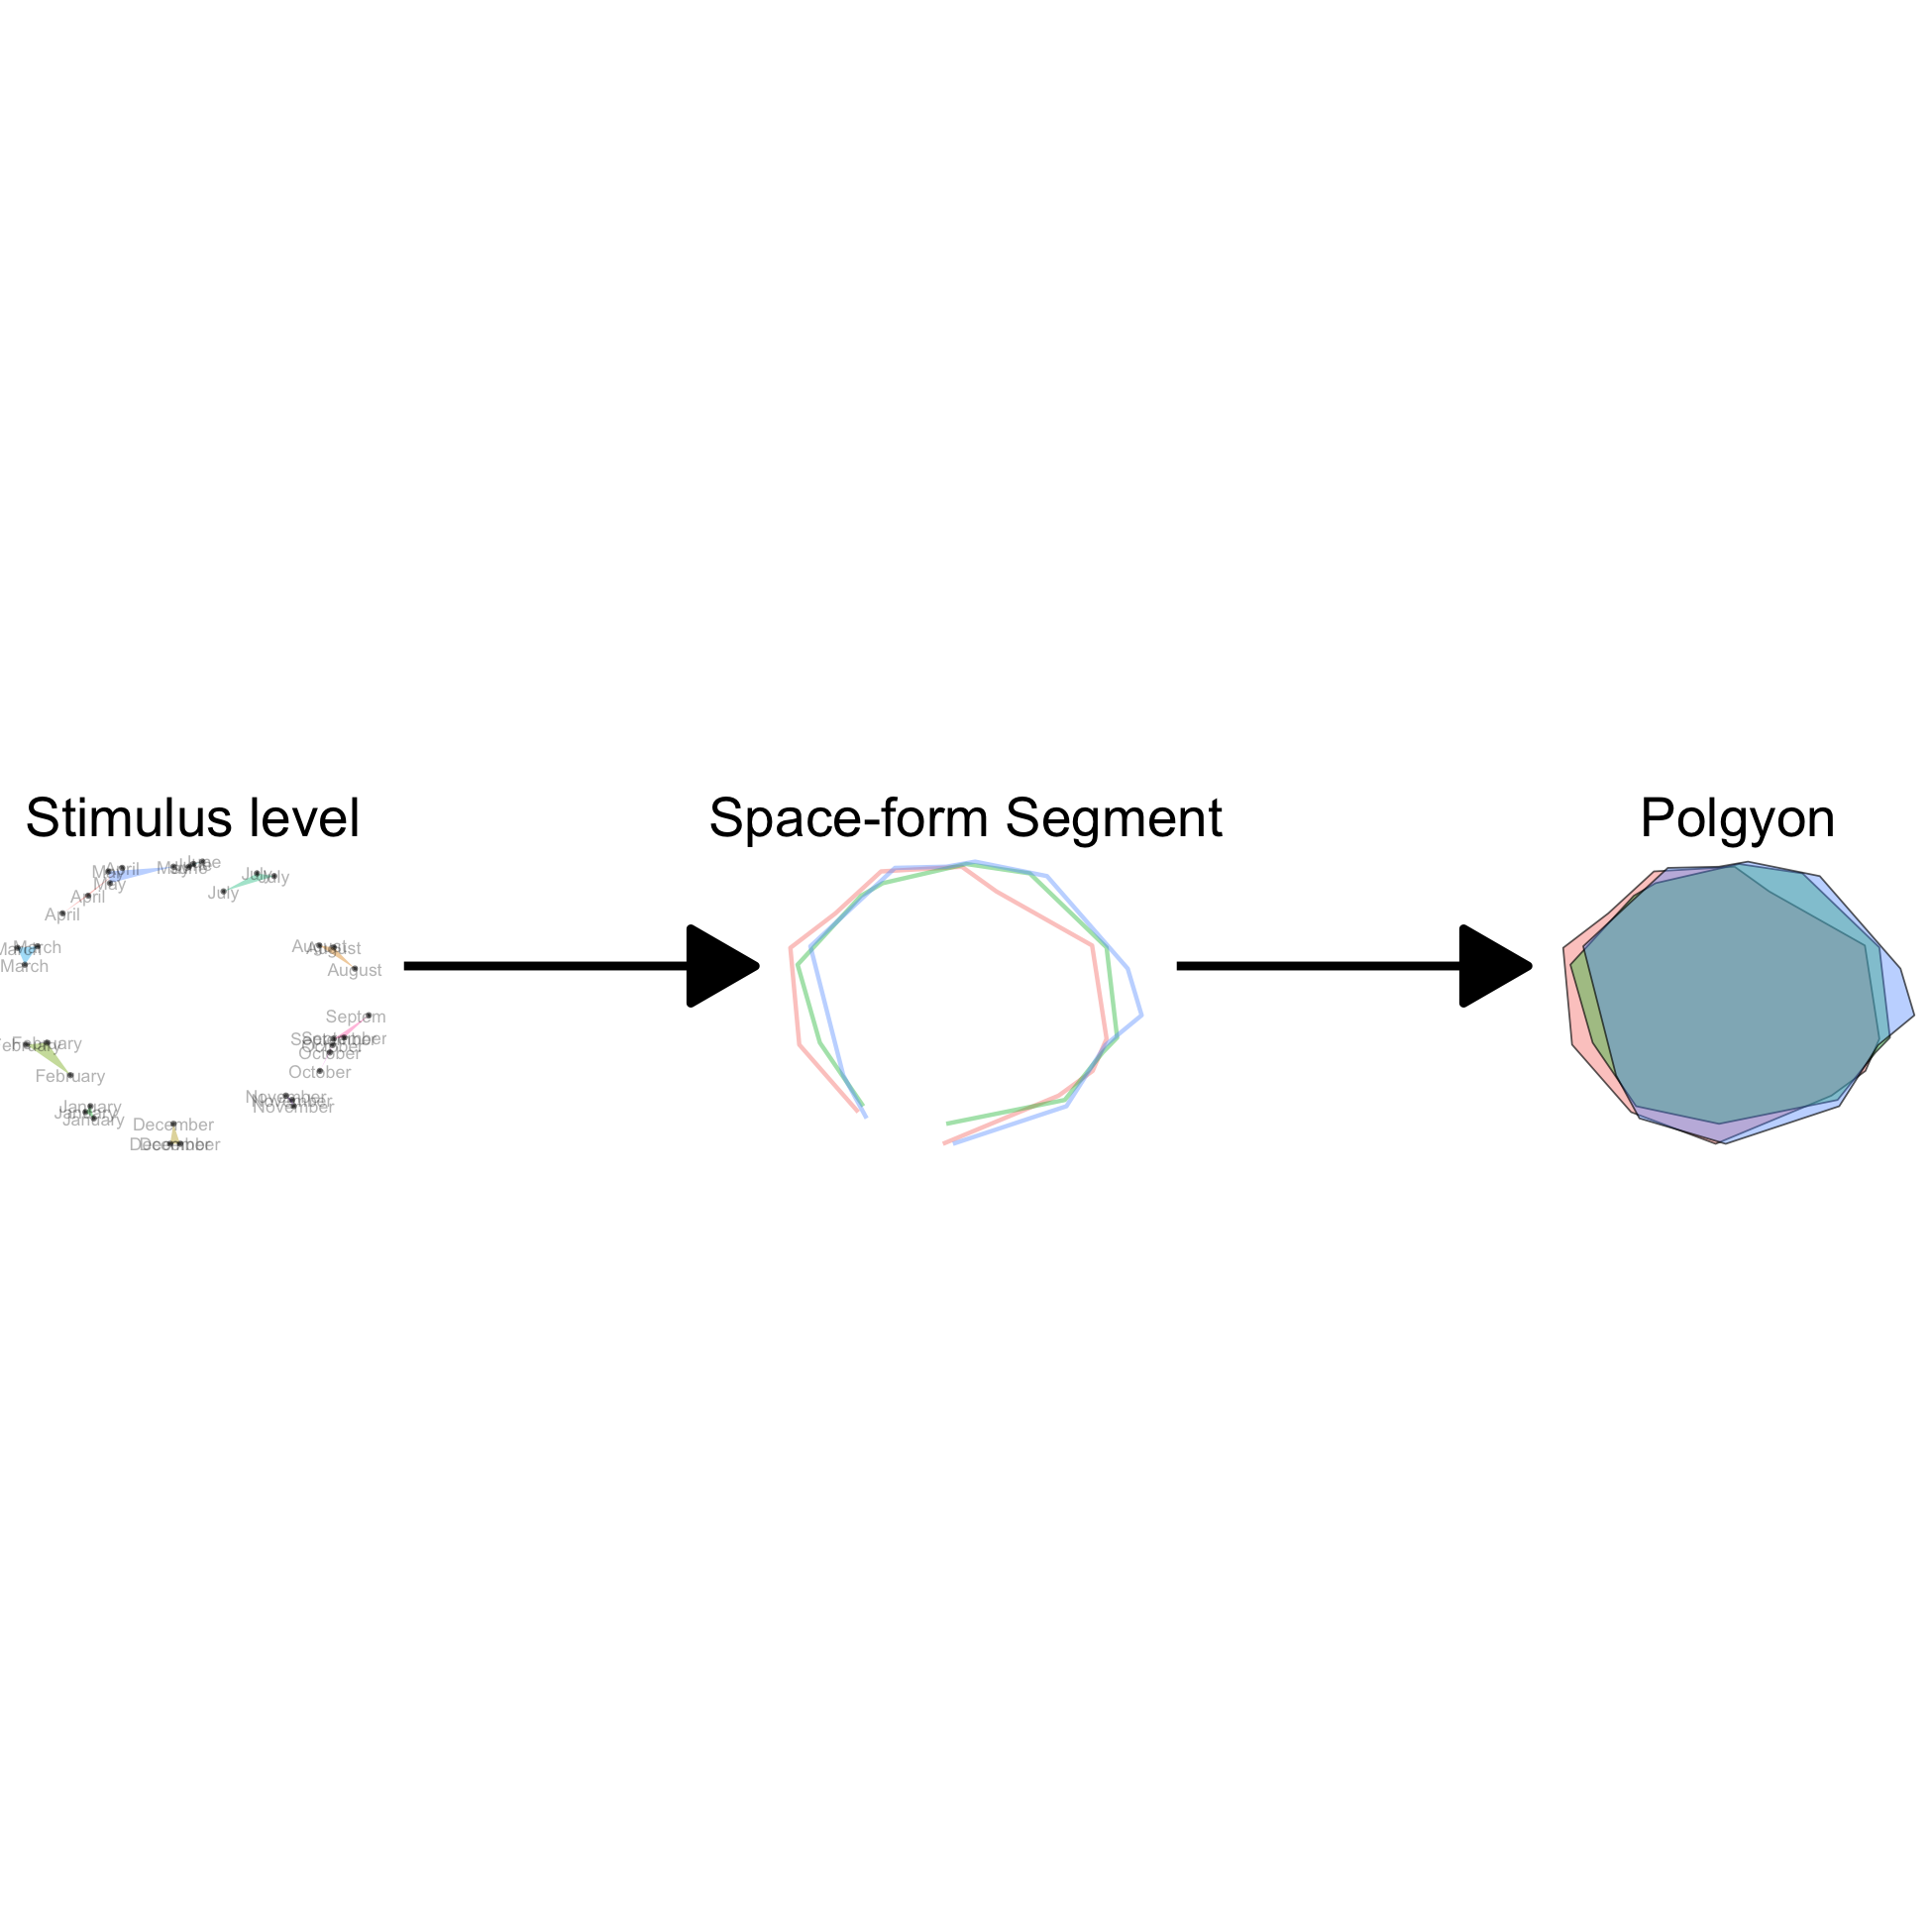
\includegraphics[keepaspectratio]{2.RegisteredReport_MS2_files/figure-pdf/fig-myplot00-1.png}}

\vspace{-20pt}
\noindent \emph{Note.} Example~participant for months

\end{figure}

\section{Results}\label{sec-results}

\begin{figure}[!htbp]

{\caption{{Receiver Operating Characteristic (ROC) curves of all
tests}{\label{fig-myplot2}}}}

\pandocbounded{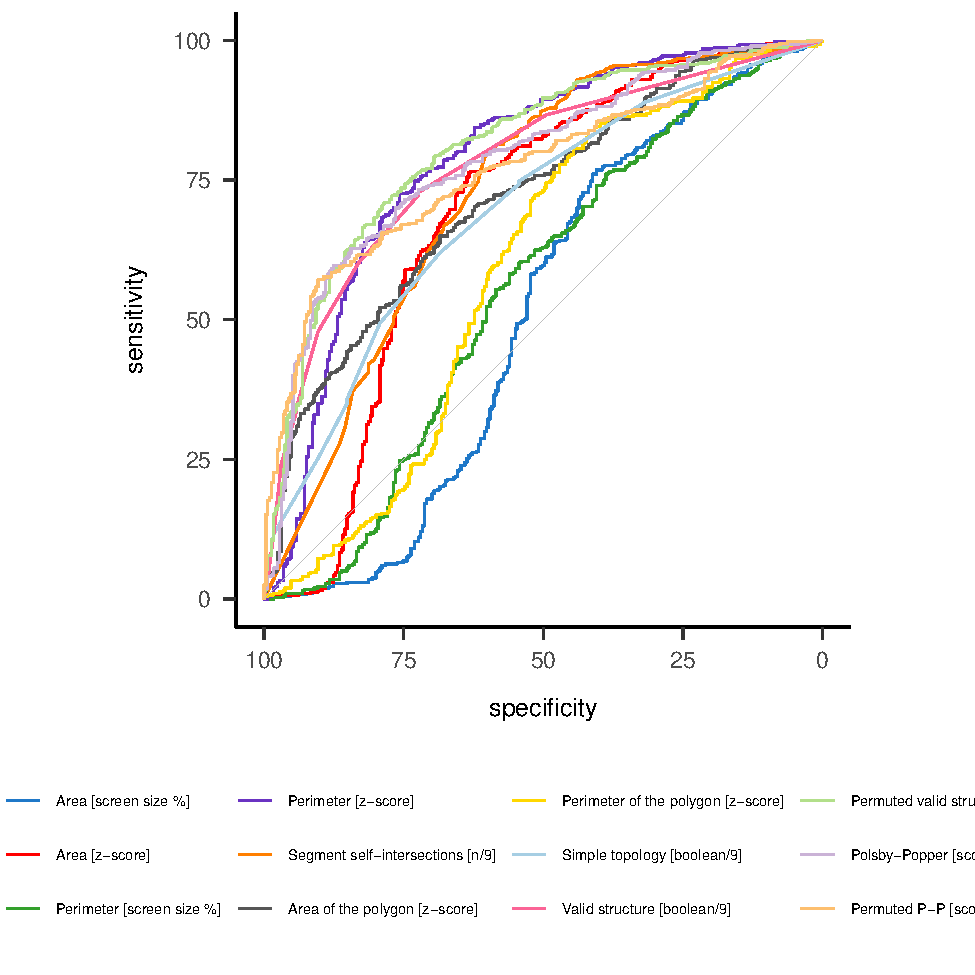
\includegraphics[keepaspectratio]{2.RegisteredReport_MS2_files/figure-pdf/fig-myplot2-1.pdf}}

\vspace{-20pt}
\noindent \emph{Note.} Grey~line indicates chance level

\end{figure}

\begin{table}

{\caption{{ROC analyses of all tests}{\label{tbl-mytb03}}}
\vspace{-20pt}}

\begin{longtable}[]{@{}
  >{\raggedright\arraybackslash}p{(\linewidth - 12\tabcolsep) * \real{0.0353}}
  >{\raggedright\arraybackslash}p{(\linewidth - 12\tabcolsep) * \real{0.4353}}
  >{\raggedleft\arraybackslash}p{(\linewidth - 12\tabcolsep) * \real{0.0706}}
  >{\raggedleft\arraybackslash}p{(\linewidth - 12\tabcolsep) * \real{0.0588}}
  >{\raggedleft\arraybackslash}p{(\linewidth - 12\tabcolsep) * \real{0.1176}}
  >{\raggedleft\arraybackslash}p{(\linewidth - 12\tabcolsep) * \real{0.1412}}
  >{\raggedleft\arraybackslash}p{(\linewidth - 12\tabcolsep) * \real{0.1412}}@{}}
\toprule\noalign{}
\begin{minipage}[b]{\linewidth}\raggedright
\end{minipage} & \begin{minipage}[b]{\linewidth}\raggedright
Feature
\end{minipage} & \begin{minipage}[b]{\linewidth}\raggedleft
AUC
\end{minipage} & \begin{minipage}[b]{\linewidth}\raggedleft
DP
\end{minipage} & \begin{minipage}[b]{\linewidth}\raggedleft
threshold
\end{minipage} & \begin{minipage}[b]{\linewidth}\raggedleft
sensitivity
\end{minipage} & \begin{minipage}[b]{\linewidth}\raggedleft
specificity
\end{minipage} \\
\midrule\noalign{}
\endhead
\bottomrule\noalign{}
\endlastfoot
10 & Permuted valid structure {[}boolean/9{]} & 81.16 & 2.13 & 0.17 &
70.78 & 78.55 \\
11 & Polsby--Popper {[}score/9{]} & 78.89 & 2.29 & 0.19 & 59.70 &
87.54 \\
4 & Perimeter {[}z-score{]} & 78.80 & 2.06 & 1.73 & 72.54 & 75.78 \\
9 & Valid structure {[}boolean/9{]} & 78.12 & 1.90 & 0.14 & 72.80 &
72.32 \\
12 & Permuted P-P {[}score/9{]} & 77.15 & 2.46 & 0.20 & 57.18 & 90.31 \\
5 & Segment self-intersections {[}n/9{]} & 72.93 & 1.75 & 1.17 & 79.85 &
60.21 \\
6 & Area of the polygon {[}z-score{]} & 72.03 & 1.36 & 1.29 & 64.99 &
68.51 \\
8 & Simple topology {[}boolean/9{]} & 69.74 & 1.24 & 0.28 & 61.96 &
68.51 \\
2 & Area {[}z-score{]} & 69.27 & 1.68 & 0.08 & 76.32 & 63.32 \\
7 & Perimeter of the polygon {[}z-score{]} & 59.12 & 1.29 & 10.46 &
83.88 & 41.87 \\
3 & Perimeter {[}screen size \%{]} & 55.34 & 0.68 & 0.03 & 76.07 &
38.75 \\
1 & Area {[}screen size \%{]} & 50.87 & 0.79 & 0.21 & 76.83 & 40.48 \\
\end{longtable}

\end{table}

\begin{table}

{\caption{{Descriptives of each test}{\label{tbl-mytb04}}}
\vspace{-20pt}}

\begin{longtable}[]{@{}
  >{\raggedright\arraybackslash}p{(\linewidth - 8\tabcolsep) * \real{0.4205}}
  >{\raggedright\arraybackslash}p{(\linewidth - 8\tabcolsep) * \real{0.1477}}
  >{\raggedright\arraybackslash}p{(\linewidth - 8\tabcolsep) * \real{0.1364}}
  >{\raggedright\arraybackslash}p{(\linewidth - 8\tabcolsep) * \real{0.1477}}
  >{\raggedright\arraybackslash}p{(\linewidth - 8\tabcolsep) * \real{0.1477}}@{}}
\toprule\noalign{}
\begin{minipage}[b]{\linewidth}\raggedright
Feature
\end{minipage} & \begin{minipage}[b]{\linewidth}\raggedright
Control
\end{minipage} & \begin{minipage}[b]{\linewidth}\raggedright
SSS
\end{minipage} & \begin{minipage}[b]{\linewidth}\raggedright
Control {[}zs{]}
\end{minipage} & \begin{minipage}[b]{\linewidth}\raggedright
SSS {[}zs{]}
\end{minipage} \\
\midrule\noalign{}
\endhead
\bottomrule\noalign{}
\endlastfoot
Permuted valid structure {[}boolean/9{]} & 0.12 (0.16) & 0.36 (0.25) &
-0.57 (0.64) & 0.41 (1.01) \\
Polsby--Popper {[}score/9{]} & 0.11 (0.13) & 0.27 (0.19) & -0.51 (0.69)
& 0.37 (1.03) \\
Perimeter {[}z-score{]} & 3.30 (1.72) & 1.59 (1.16) & 0.60 (1.04) &
-0.44 (0.70) \\
Valid structure {[}boolean/9{]} & 0.13 (0.19) & 0.39 (0.28) & -0.54
(0.69) & 0.39 (1.01) \\
Permuted P-P {[}score/9{]} & 0.11 (0.17) & 0.41 (0.33) & -0.56 (0.56) &
0.40 (1.06) \\
Segment self-intersections {[}n/9{]} & 9.56 (11.31) & 1.87 (5.42) & 0.48
(1.23) & -0.35 (0.59) \\
Area of the polygon {[}z-score{]} & 1.00 (0.99) & 1.91 (1.31) & -0.42
(0.79) & 0.30 (1.03) \\
Simple topology {[}boolean/9{]} & 0.22 (0.23) & 0.40 (0.27) & -0.39
(0.85) & 0.28 (1.01) \\
Area {[}z-score{]} & 0.26 (0.32) & 0.08 (0.14) & 0.42 (1.29) & -0.30
(0.55) \\
Perimeter of the polygon {[}z-score{]} & 9.49 (3.44) & 8.39 (2.48) &
0.21 (1.16) & -0.16 (0.83) \\
Perimeter {[}screen size \%{]} & 0.03 (0.03) & 0.03 (0.08) & 0.03 (0.44)
& -0.02 (1.26) \\
Area {[}screen size \%{]} & 0.46 (0.87) & 0.26 (0.52) & 0.17 (1.25) &
-0.12 (0.75) \\
\end{longtable}

\end{table}

Descriptively, the triangle area (in \% screen size) between repetition
for SSS was surprisingly larger than in previous studies: 0.26\%
(\emph{SD = 0.52\%}) compared to 0.15\% (\emph{SD = 0.13 \%}) in Rothen
et al. (\citeproc{ref-rothen2016}{2016}) and 0.14 \% (\emph{SD = 0.17})
\% in Ward et al. (\citeproc{ref-ward2018}{2018}), see
Table~\ref{tbl-mytb04}. These values also differ between the available
datasets (See Figure~\ref{fig-apx08}). However, those differences could
be mitigated by using individually standardized coordinates, see
Table~\ref{tbl-mytb04}.

\subsection{ROC analyses}\label{roc-analyses}

All ROC were compared to the permuted validity method, since it led the
highest AUC (81.16), all p-values false discovery rate (FDR) adjusted.
ROC analyses are summarized in Table~\ref{tbl-mytb03} and
Figure~\ref{fig-myplot2}. Interestingly, while the permuted validity
leads to significantly larger AUC than the Polsby-Popper method,
(\emph{D} = 2.14 , \emph{p} \textless{} .05, it led to similar AUC than
the standardized perimeter (\emph{D} = 1.4, \emph{p} \textless{} .05).
This might be explained by the relatively lower sensitivity 59.7
(although relatively higher sensitivity 87.54) of the Polsby-Popper test
compared to the Perimeter (72.54) and permuted validity tests (70.78).
Additionally, the permuted validity led to significantly higher AUC than
the non permuted one (D = 3.12, \emph{p} \textless{} .05).

Hence, the two best AUC performances are from the averaged permuted
validity score (AUC = 81.16; DP = 2.13, cut-off = 0.17 corresponding to
1.53 valid of 9 forms) and the standardized perimeter between the
repetitions of each stimuli (AUC = 78.8; DP = 2.06, cut-off = 1.73
z-scores). At the proposed cut-off, the permuted validity leads to
higher specificity than perimeter (78.55 vs. 75.78) indicating better
rejection of controls (i.e.~less false negatives), but lower sensitivity
(70.78 vs. 72.54), indicating poorer detection of SSS (i.e.~more false
negatives).

In sum, the permuted validity on the space-form level and the perimeter
of standardized coordinates on the stimulus level were the two equally
optimal tests to classify controls and SSS.

\subsection{Further analyses}\label{further-analyses}

We conducted further analyses by subsampling the dataset source and
questionnaire percentiles. The aim of these analyses was to test the
stability of the classifications from different methods across
experiments (i.e.~datasets) and sample characteristics (i.e.
questionnaire scores). We also used a correlational approach to test for
correlations between features and questionnaires.

We sub-sampled the dataset source for the five most optimal tests (i.e.
higher AUC) and recalculated AUC, sensitivity and sensibility. We found
similar values for the different datasets, see
Figure~\ref{fig-myplotapx02}.

Including only the data by Professor Ward, we subsampled the
participants depending on the perecntiles of the questionnaire scores
(hence only the data from Professor Ward), taking the 10-0\% highest
questionnaire scores against the 10 \% lowest (. (i.e.~90-100 \%). Here
also most of the values remain relatively stable independently from the
questionnaire distribution of the samples, see
Figure~\ref{fig-myplotapx03}. Another important point addressed in the
literature about consistency test is circularity. The circularity is
given in that if consistency tests are used to classify SSS and
controls, then those groups will by definition differ in consistency
(\citeproc{ref-root2025}{Root et al., 2025}). Hence, we made a
correlation matrix with the questionnaire scores and all the tests, see
Appendix. The two highest correlations are indeed between the
questionnaire score and perimeter (r = .58) and permuted validity (r =
.50), see Figure~\ref{fig-myplotapx04}.

Some of the participants might have been originally mis-attributed to
control or SSS or there might be consistent controls and inconsistent
synesthetes (\citeproc{ref-eagleman2007}{Eagleman et al., 2007}; see
\citeproc{ref-root2025}{Root et al., 2025}). We found about
\textasciitilde6 \% of the full sample's synesthetes to be consistently
classified as controls (i.e.~consistent false positive) by the five
methods with the highest AUC, see , see Figure~\ref{fig-myplotapx07} and
Figure~\ref{fig-myplotapx08}. \textasciitilde3 \% controls are
consistently classified as SSS (i.e.~consistent false negative)
Figure~\ref{fig-myplotapx09}.

Finally, we also wanted to visualize the average space form of each
category at the population level to see if there were qualitative
differences between the forms. The figure in the appendix
(Figure~\ref{fig-myplotapx06}), shows more circular patterns for months
and more linear horizontal and vertical for numbers.

\section{Methods - future study}\label{sec-phase-ii-methods}

Additional data will be collected in the future using the same
consistency test, with the procedural exception that there will be four
repetitions per stimuli instead of three ( Sachdeva et al.
(\citeproc{ref-sachdeva2024}{2024}), Stage 1 in-principle acceptance).
Hence for the stimulus levels tests we will compare the area and
perimeter of a quadrilateral of four coordinates pairs instead of a
triangle. Materials are more details on this study are pre-registered on
OSF, including ample size and recruitment method
(\citeproc{ref-sachdeva2024}{Sachdeva et al., 2024}, Stage 1
in-principle acceptance) (see also \url{https://osf.io/6wn4m}).

We will compute the same ROC analyses as in this pre-registration on all
the tests. Since we obtain different best AUC per tests depending on the
dataset (see Figure~\ref{fig-myplotapx02}) it is likely that the best
test here will not match with the best test in the to be collected
dataset.

\section{Discussion - present study}\label{discussion---present-study}

Our investigation of four datasets found two main consistency tests
leading to the optimal classification of SSS from control: standardized
perimeter between stimulus repetitions and permuted topological validity
on the space-form level.

Further analyses show variabilities between the test's AUC exists
depending on the dataset source, which could explain why we could not
replicate Rothen et al. (\citeproc{ref-rothen2016}{2016})'s area but
rather found the perimeter as a more optimal test. The stability across
varying percentiles of the synesthesia questionnaire's score suggest the
tests work as well for more marked forms of SSS (note however that this
analysis was limited Professor Ward's data). The standardized perimeter
also leads to slightly higher correlation with the questionnaire scores
(r = .57) than permuted topological validity (r = .51), see
Figure~\ref{fig-myplotapx04}.

In sum, while we could prove similar performances using a different
approach based on the space-form level (i.e.~topological validity), we
found similar classification performances than using stimulus-repetition
level test such as perimeter.

\subsection{Limitations}\label{sec-limitations}

Although an optimal test to classify SSS might be particularly relevant
for experimental purposes, several important limitations need to be
considered. First, consistency tests contain only a limited set of
sequential stimuli (i.e.~months, weeks and the first ten natural
numbers) that could potentially elicit synaesthetic experiences. Other
ordinal categories such as temperature, clock time, musical keys might
be more relevant for some individuals with SSS. For numbers
specifically, better consistency tests might be obtained using a larger
set size (i.e.~including decades and hundreds), as descriptively
interesting form changes occur at different decimals in base-10 number
systems (\citeproc{ref-galton1880}{Galton, 1880}).

Second, the use of diagnostic cutoffs assumes categorical distinctions
between groups, but SSS may exist on a continuum and scores might be
more suitable (\citeproc{ref-price2013}{Price \& Pearson, 2013}). This
limitation is related to the circularity mentioned previously:
diagnostic cutoffs as calculated here depend on how SSS and controls are
classified in the first place (\citeproc{ref-simner2012}{Simner, 2012}).
Measures of other characteristics of synaesthesia such as automaticity
or visual Gabor detection might be necessary to establish external
validity (\citeproc{ref-ward2018}{Ward et al., 2018}). Indeed,
determining the prevalence of SSS in the general population requires
definitional choices that might be based on more conservative or lenient
criteria (\citeproc{ref-brang2010}{Brang et al., 2010};
\citeproc{ref-jonas2014}{Jonas \& Price, 2014};
\citeproc{ref-sagiv2006}{Sagiv et al., 2006};
\citeproc{ref-ward2018}{Ward et al., 2018}). These difficulties are
reflected in the span of current prevalence estimates of SSS: 4.4 \%
(\citeproc{ref-brang2013}{Brang et al., 2013}), 8.1 \%
(\citeproc{ref-ward2018}{Ward et al., 2018}) and 14 \%
(\citeproc{ref-seron1992}{Seron et al., 1992}).

Third, as shown in Figure~\ref{fig-myplotapx02}, we find that the
optimal criteria can vary across datasets. In other word, we obtain
different AUC depending on the datasets. These differences might be
explained by different sampling methods biases, for example
(\citeproc{ref-vanpetersen2020}{Van Petersen et al., 2020}) recruited
SSS from over one hundred candidates to maximise participant reporting
synesthetic experiences.

\subsection{Topological validity}\label{topological-validity}

Surprisingly, permuted topological validity of the spatial-forms led to
similar results than the perimeter test. This novel result might be
informative about how SSS map ordinal stimuli in space. Indeed, it seems
the patterns of spatial-forms follow topological rules analogous to
geographical and geometry-based space structures. Analogies between maps
and neuroscience have a long history (i.e.~retinotopy, sonotopy or
somatotopy \citeproc{ref-eagleman2009}{Eagleman \& Goodale, 2009}).
Therefore spatial-forms might originate from the mapping between ordinal
or sequential stimuli on idiosyncratic visuo-spatial abilities following
topological rules. One of the advantages of using topological validity
is that it also classifies responses with the same coordinates as
invalid and hence inconsistent, while using the area and perimeter
metrics they would qualify as highly consistent responses.

\subsection{Intermediary Conclusion}\label{sec-conclusions}

The present study compared traditional stimulus-level consistency tests
with novel form-level geometric tests for detecting SSS. We found
optimal classification performance from permuted topological validity
and standardized perimeter between repetitions. Despite not yielding to
better classification than stimulus level methods, this new method is
theoretically meaningful since genuine synesthetes should produce more
compact and topologically valid structures compared to controls.
Similarly, the perimeter test captures the stability of the overall
spatial configuration across repetitions, which should remain consistent
for true SSS individuals regardless of presentation order.

In the future study, we will attempt at validating these criteria on a
yet-to be acquired dataset.

\section{References}\label{references}

\phantomsection\label{refs}
\begin{CSLReferences}{1}{0}
\bibitem[\citeproctext]{ref-baron-cohen1993}
Baron-Cohen, S., Harrison, J., Goldstein, L. H., \& Wyke, M. (1993).
Coloured Speech Perception: Is Synaesthesia what Happens when Modularity
Breaks Down? \emph{Perception}, \emph{22}(4), 419--426.
\url{https://doi.org/10.1068/p220419}

\bibitem[\citeproctext]{ref-brang2013}
Brang, D., Miller, L. E., McQuire, M., Ramachandran, V. S., \& Coulson,
S. (2013). Enhanced mental rotation ability in time-space synesthesia.
\emph{Cognitive Processing}, \emph{14}(4), 429--434.
\url{https://doi.org/10.1007/s10339-013-0561-5}

\bibitem[\citeproctext]{ref-brang2010}
Brang, D., Teuscher, U., Ramachandran, V. S., \& Coulson, S. (2010).
Temporal sequences, synesthetic mappings, and cultural biases: The
geography of time. \emph{Consciousness and Cognition}, \emph{19}(1),
311--320. \url{https://doi.org/10.1016/j.concog.2010.01.003}

\bibitem[\citeproctext]{ref-ggalluvial}
Brunson, J. C., \& Read, Q. D. (2023). \emph{{ggalluvial}: Alluvial
plots in 'ggplot2'}. \url{http://corybrunson.github.io/ggalluvial/}

\bibitem[\citeproctext]{ref-deroy2013}
Deroy, O., \& Spence, C. (2013). Why we are not all synesthetes (not
even weakly so). \emph{Psychonomic Bulletin \& Review}, \emph{20}(4),
643--664. \url{https://doi.org/10.3758/s13423-013-0387-2}

\bibitem[\citeproctext]{ref-dixon2004}
Dixon, M. J., Smilek, D., \& Merikle, P. M. (2004). Not all synaesthetes
are created equal: Projector versus associator synaesthetes.
\emph{Cognitive, Affective, \& Behavioral Neuroscience}, \emph{4}(3),
335--343. \url{https://doi.org/10.3758/CABN.4.3.335}

\bibitem[\citeproctext]{ref-eagleman2009a}
Eagleman, D. M. (2009). The objectification of overlearned sequences: A
new view of spatial sequence synesthesia. \emph{Cortex}, \emph{45}(10),
1266--1277. \url{https://doi.org/10.1016/j.cortex.2009.06.012}

\bibitem[\citeproctext]{ref-eagleman2009}
Eagleman, D. M., \& Goodale, M. A. (2009). Why color synesthesia
involves more than color. \emph{Trends in Cognitive Sciences},
\emph{13}(7), 288--292. \url{https://doi.org/10.1016/j.tics.2009.03.009}

\bibitem[\citeproctext]{ref-eagleman2007}
Eagleman, D. M., Kagan, A. D., Nelson, S. S., Sagaram, D., \& Sarma, A.
K. (2007). A standardized test battery for the study of synesthesia.
\emph{Journal of Neuroscience Methods}, \emph{159}(1), 139--145.
\url{https://doi.org/10.1016/j.jneumeth.2006.07.012}

\bibitem[\citeproctext]{ref-flournoy1893}
Flournoy, T. (1893). \emph{Des phénomènes de synopsie (audition
colorée): Photismes, schèmes visuels, personnifications}. Alcan.
\url{https://books.google.bj/books?id=JISQxpcyGUMC}

\bibitem[\citeproctext]{ref-galton1880}
Galton, F. (1880). Visualised Numerals. \emph{Nature}, \emph{21}(533),
252--256. \url{https://doi.org/10.1038/021252a0}

\bibitem[\citeproctext]{ref-ggVennDiagram}
Gao, C.-H., \& Dusa, A. (2025). \emph{{ggVennDiagram}: A 'ggplot2'
implement of venn diagram}.
\url{https://github.com/gaospecial/ggVennDiagram}

\bibitem[\citeproctext]{ref-gould2014}
Gould, C., Froese, T., Barrett, A. B., Ward, J., \& Seth, A. K. (2014).
An extended case study on the phenomenology of sequence-space
synesthesia. \emph{Frontiers in Human Neuroscience}, \emph{8}.
\url{https://doi.org/10.3389/fnhum.2014.00433}

\bibitem[\citeproctext]{ref-herring2010}
Herring, J. R. (2010). \emph{OpenGIS® Implementation Standard for
Geographic information - Simple feature access - Part 1: Common
architecture}.

\bibitem[\citeproctext]{ref-jarick2009}
Jarick, M., Dixon, M. J., Stewart, M. T., Maxwell, E. C., \& Smilek, D.
(2009). A different outlook on time: Visual and auditory month names
elicit different mental vantage points for a time-space synaesthete.
\emph{Cortex}, \emph{45}(10), 1217--1228.
\url{https://doi.org/10.1016/j.cortex.2009.05.014}

\bibitem[\citeproctext]{ref-jonas2014}
Jonas, C. N., \& Price, M. C. (2014). Not all synesthetes are alike:
Spatial vs. Visual dimensions of sequence-space synesthesia.
\emph{Frontiers in Psychology}, \emph{5}.
\url{https://doi.org/10.3389/fpsyg.2014.01171}

\bibitem[\citeproctext]{ref-lyons2013}
Lyons, I. M., \& Beilock, S. L. (2013). Ordinality and the Nature of
Symbolic Numbers. \emph{The Journal of Neuroscience}, \emph{33}(43),
17052--17061. \url{https://doi.org/10.1523/JNEUROSCI.1775-13.2013}

\bibitem[\citeproctext]{ref-sf}
Pebesma, E., \& Bivand, R. (2023). \emph{{Spatial Data Science: With
applications in {R}}}. {Chapman and Hall/CRC}.
\url{https://doi.org/10.1201/9780429459016}

\bibitem[\citeproctext]{ref-polsby1991}
Polsby, D. D., \& Popper, R. (1991). The Third Criterion: Compactness as
a Procedural Safeguard Against Partisan Gerrymandering. \emph{SSRN
Electronic Journal}. \url{https://doi.org/10.2139/ssrn.2936284}

\bibitem[\citeproctext]{ref-postgis}
\emph{PostGIS 3.6.2dev manual}. (n.d.).

\bibitem[\citeproctext]{ref-price2013}
Price, M., \& Pearson, D. (2013). Toward a visuospatial developmental
account of sequence-space synesthesia. \emph{Frontiers in Human
Neuroscience}, \emph{7}. \url{https://doi.org/10.3389/fnhum.2013.00689}

\bibitem[\citeproctext]{ref-pROC}
Robin, X., Turck, N., Hainard, A., Tiberti, N., Lisacek, F., Sanchez,
J.-C., \& Müller, M. (2011). {pROC}: An open-source package for {R} and
{S}+ to analyze and compare ROC curves. \emph{BMC Bioinformatics},
\emph{12}, 77.

\bibitem[\citeproctext]{ref-root2021}
Root, N., Asano, M., Melero, H., Kim, C.-Y., Sidoroff-Dorso, A. V.,
Vatakis, A., Yokosawa, K., Ramachandran, V., \& Rouw, R. (2021). Do the
colors of your letters depend on your language? Language-dependent and
universal influences on grapheme-color synesthesia in seven languages.
\emph{Consciousness and Cognition}, \emph{95}, 103192.
\url{https://doi.org/10.1016/j.concog.2021.103192}

\bibitem[\citeproctext]{ref-root2025}
Root, N., Chkhaidze, A., Melero, H., Sidoroff-Dorso, A., Volberg, G.,
Zhang, Y., \& Rouw, R. (2025). How {``}diagnostic{''} criteria interact
to shape synesthetic behavior: The role of self-report and
test{\textendash}retest consistency in synesthesia research.
\emph{Consciousness and Cognition}, \emph{129}, 103819.
\url{https://doi.org/10.1016/j.concog.2025.103819}

\bibitem[\citeproctext]{ref-rothen2016}
Rothen, N., Jünemann, K., Mealor, A. D., Burckhardt, V., \& Ward, J.
(2016). The sensitivity and specificity of a diagnostic test of
sequence-space synesthesia. \emph{Behavior Research Methods},
\emph{48}(4), 1476--1481.
\url{https://doi.org/10.3758/s13428-015-0656-2}

\bibitem[\citeproctext]{ref-rothen2013a}
Rothen, N., Seth, A. K., Witzel, C., \& Ward, J. (2013). Diagnosing
synaesthesia with online colour pickers: Maximising sensitivity and
specificity. \emph{Journal of Neuroscience Methods}, \emph{215}(1),
156--160. \url{https://doi.org/10.1016/j.jneumeth.2013.02.009}

\bibitem[\citeproctext]{ref-sachdeva2024}
Sachdeva, C., Whelan, E., Ovalle-Fresa, R., Rey-Mermet, A., Ward, J., \&
Rothen, N. (2024). \emph{How perceptual ability shapes memory: An
investigation in healthy special populations}.
\url{https://osf.io/6wn4m}

\bibitem[\citeproctext]{ref-sagiv2006}
Sagiv, N., Simner, J., Collins, J., Butterworth, B., \& Ward, J. (2006).
What is the relationship between synaesthesia and visuo-spatial number
forms? \emph{Cognition}, \emph{101}(1), 114--128.
\url{https://doi.org/10.1016/j.cognition.2005.09.004}

\bibitem[\citeproctext]{ref-seron1992}
Seron, X., Pesenti, M., Noël, M.-P., Deloche, G., \& Cornet, J.-A.
(1992). Images of numbers, or {``}when 98 is upper left and 6 sky
blue{''}. \emph{Cognition}, \emph{44}(1), 159--196.
\url{https://doi.org/10.1016/0010-0277(92)90053-K}

\bibitem[\citeproctext]{ref-simner2012}
Simner, J. (2012). Defining synaesthesia. \emph{British Journal of
Psychology}, \emph{103}(1), 1--15.
\url{https://doi.org/10.1348/000712610X528305}

\bibitem[\citeproctext]{ref-smilek2007}
Smilek, D., Callejas, A., Dixon, M. J., \& Merikle, P. M. (2007). Ovals
of time: Time-space associations in synaesthesia. \emph{Consciousness
and Cognition}, \emph{16}(2), 507--519.
\url{https://doi.org/10.1016/j.concog.2006.06.013}

\bibitem[\citeproctext]{ref-vanpetersen2020}
Van Petersen, E., Altgassen, M., Van Lier, R., \& Van Leeuwen, T. M.
(2020). Enhanced spatial navigation skills in sequence-space
synesthetes. \emph{Cortex}, \emph{130}, 49--63.
\url{https://doi.org/10.1016/j.cortex.2020.04.034}

\bibitem[\citeproctext]{ref-ward2022a}
Ward, J. (2022). \emph{Optimizing a measure of consistency for
sequence-space synaesthesia}. \url{https://osf.io/5cnr7_v1}

\bibitem[\citeproctext]{ref-ward2018}
Ward, J., Ipser, A., Phanvanova, E., Brown, P., Bunte, I., \& Simner, J.
(2018). The prevalence and cognitive profile of sequence-space
synaesthesia. \emph{Consciousness and Cognition}, \emph{61}, 79--93.
\url{https://doi.org/10.1016/j.concog.2018.03.012}

\bibitem[\citeproctext]{ref-ward2022}
Ward, J., \& Simner, J. (2022). How do Different Types of Synesthesia
Cluster Together? Implications for Causal Mechanisms. \emph{Perception},
\emph{51}(2), 91--113. \url{https://doi.org/10.1177/03010066211070761}

\bibitem[\citeproctext]{ref-corrplot}
Wei, T., \& Simko, V. (2024). \emph{R package '{corrplot}':
Visualization of a correlation matrix}.
\url{https://github.com/taiyun/corrplot}

\bibitem[\citeproctext]{ref-ggplot2}
Wickham, H. (2016). \emph{{ggplot2}: Elegant graphics for data
analysis}. Springer-Verlag New York. \url{https://ggplot2.tidyverse.org}

\bibitem[\citeproctext]{ref-cowplot}
Wilke, C. O. (2025a). \emph{{cowplot}: Streamlined plot theme and plot
annotations for 'ggplot2'}.
\url{https://doi.org/10.32614/CRAN.package.cowplot}

\bibitem[\citeproctext]{ref-ggridges}
Wilke, C. O. (2025b). \emph{{ggridges}: Ridgeline plots in 'ggplot2'}.
\url{https://doi.org/10.32614/CRAN.package.ggridges}

\bibitem[\citeproctext]{ref-youden1950}
Youden, W. J. (1950). Index for rating diagnostic tests. \emph{Cancer},
\emph{3}(1), 32--35.
\url{https://doi.org/10.1002/1097-0142(1950)3:1\%3C32::aid-cncr2820030106\%3E3.0.co;2-3}

\end{CSLReferences}

\newpage{}

\subsubsection{Appendix}\label{appendix}

The additional analyses in this appendix attempt to address several
concerns. Regarding the distribution's of the scores from the different
methods, i.e.~whether it is bimodal, see
\hyperref[apx-featDensity]{Appendix~A}. Then to visualize the stability
of the ROC analyses across the datasets, i.e. whether AUC, DP,
sensitivity and specificity vary across the four different datasets, see
\hyperref[apx-SM2byds]{Appendix~B}.

To address circularity concerns that we might find methods that best
classifies synesthetes and controls only from the sed on self-reported
groups, we attempted two additional approaches: first, testing
sub-samples based on percentiles of the questionnaire score sample
distribution (see \hyperref[apx-byquestperc]{Appendix~C}). The rationale
is that a good consistency test should have similar discriminative
performance for strong SSS and weaker SSS. To do this, we re-sampled the
SSS and controls based on their questionnaire distribution by
percentiles (i.e., comparing 10\% highest questionnaire scores vs.~10\%
lowest, then 20\% vs. 20\%, etc.). In addition, we correlated the
questionnaire scores with the results from different features extracted
from the consistency test, see
\hyperref[apx-correlation-with-self-report]{Appendix~D}.

We also wanted to visually characterize whether certain patterns occur
more frequently for some categories than others (i.e.~circular pattern
for months and linear for numbers).
\hyperref[apx-average-forms]{Appendix~E} shows the average forms for
each categories. Finally, we wanted to visualize how each participant is
classified by each test. From this we found a group of Synaesthetic who
consistently are classified as controls by different methods as well as
a group of control who are consistently classified as synaesthetes, see
\hyperref[apx-alluvial]{Appendix~F}.

The following R packages were used for the data visualization in the
appendix: `ggridges' v. 0.5.7 (\citeproc{ref-ggridges}{Wilke, 2025b}),
`cowplot' v. 1.2.0 (\citeproc{ref-cowplot}{Wilke, 2025a}), `ggalluvial'
v. 0.12.5 (\citeproc{ref-ggalluvial}{Brunson \& Read, 2023}), `corrplot'
v. 0.95 (\citeproc{ref-corrplot}{Wei \& Simko, 2024})

\appendix

\section{Test's distributions}\label{apx-featDensity}

Regarding the distributions of each tests across the SSS vs.~controls,
Figure~\ref{fig-apx01} we compared the density plots of each
standardized criteria (in order to make them comparable) which visually
suggests bimodal distribution.

\begin{figure}

{\caption{{Density plots of all the features comparing SSS and
controls}{\label{fig-apx01}}}}

\pandocbounded{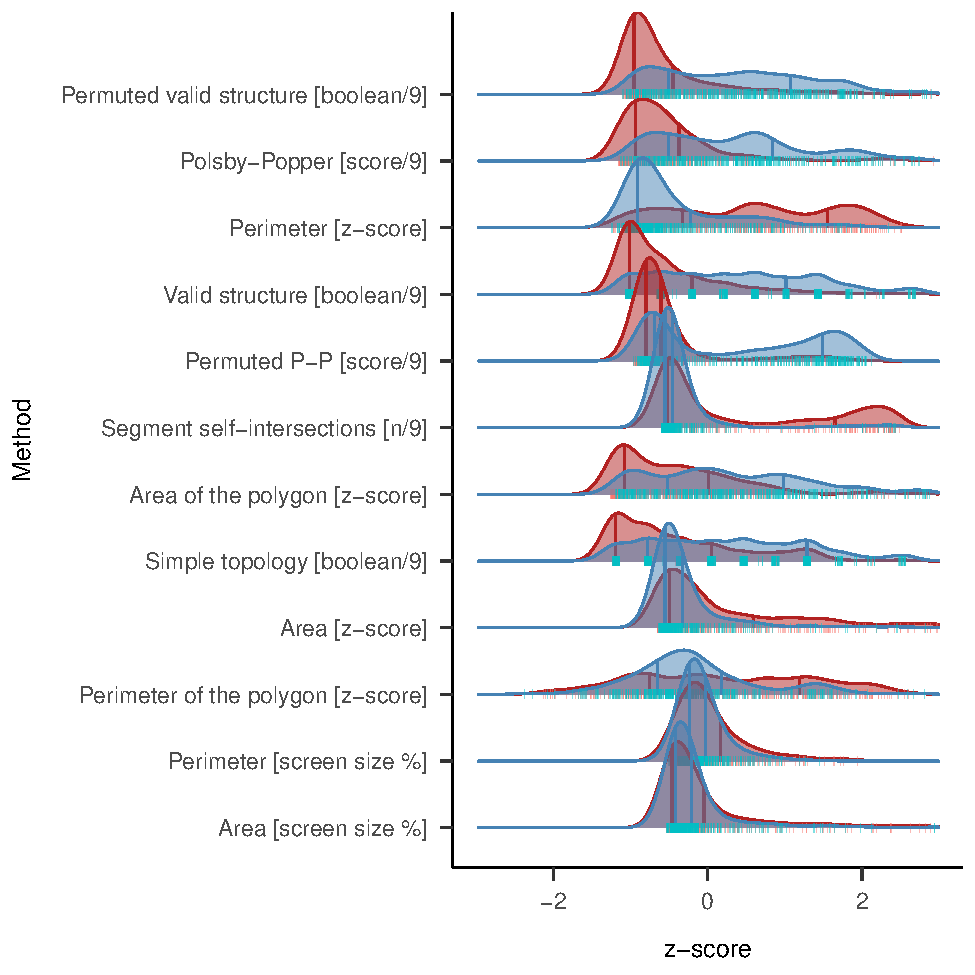
\includegraphics[keepaspectratio]{2.RegisteredReport_MS2_files/figure-pdf/fig-apx01-1.pdf}}

\vspace{-20pt}
\noindent \emph{Note.} Red~= Classified as Synesthetes, Blue = as
controls.

All method's score have been standardized (\emph{z-score}). x axis
treamed between -3 and 3 z-scores. Vertical line represent respectively
25 and 75 percentiles of each distributions.

\end{figure}

\section{ROC analysis by dataset}\label{apx-SM2byds}

Here we compare the ROC analyses results for each data sample of the
three methods with the best AUC, see Figure~\ref{fig-apx08}.
Descriptively, we also looked a the distributions of each methods across
SSS and controls Figure~\ref{fig-myplotapx02}. Note that the dataset
labelled as Ward 2 has more synaesthetes than controls (5:1 ratio). Note
that some of the tests led to 100 \% Specificity in Van Petersen et al.
(\citeproc{ref-vanpetersen2020}{2020}) dataset.

\begin{figure}

{\caption{{Lineplots of AUC and DP by data
source}{\label{fig-myplotapx02}}}}

\pandocbounded{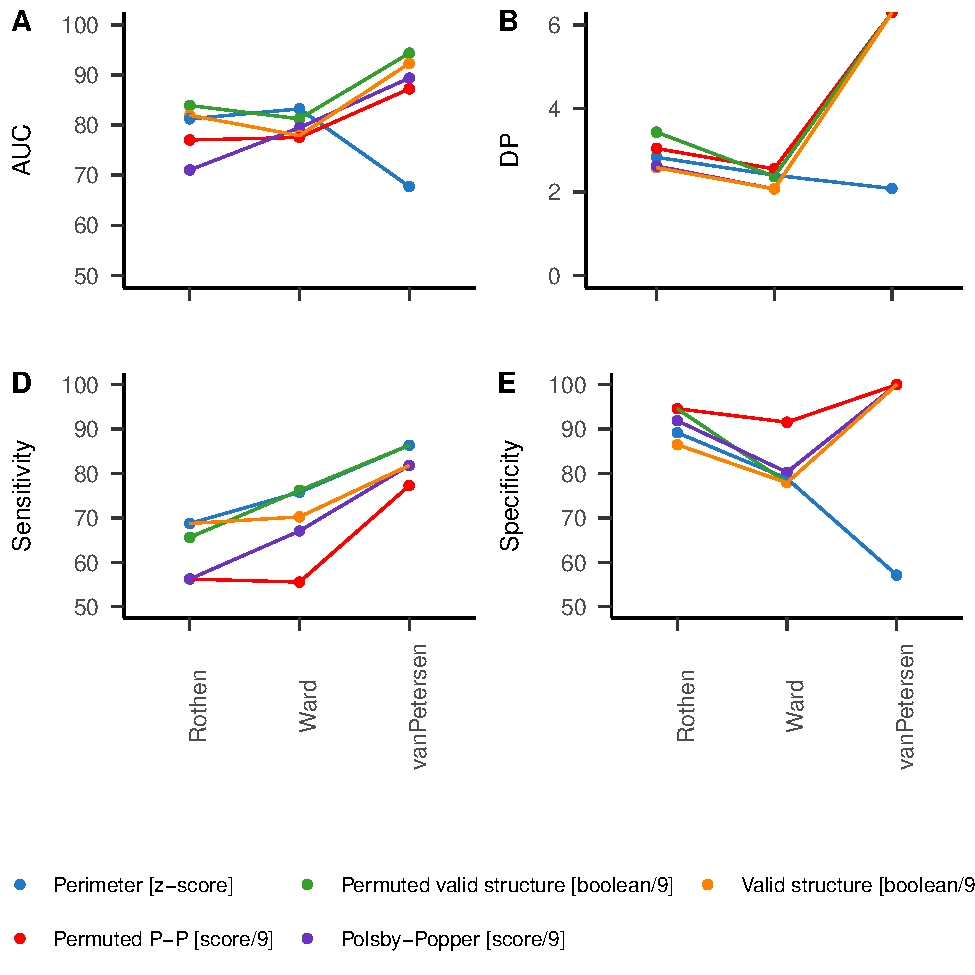
\includegraphics[keepaspectratio]{2.RegisteredReport_MS2_files/figure-pdf/fig-myplotapx02-1.pdf}}

\vspace{-20pt}
\noindent \emph{Note.} AUC~= Area Under the Curve, DP = Discrimination
Power

\end{figure}

\begin{figure}

{\caption{{Density plots of all the tests comparing SSS and controls by
dataset}{\label{fig-apx08}}}}

\pandocbounded{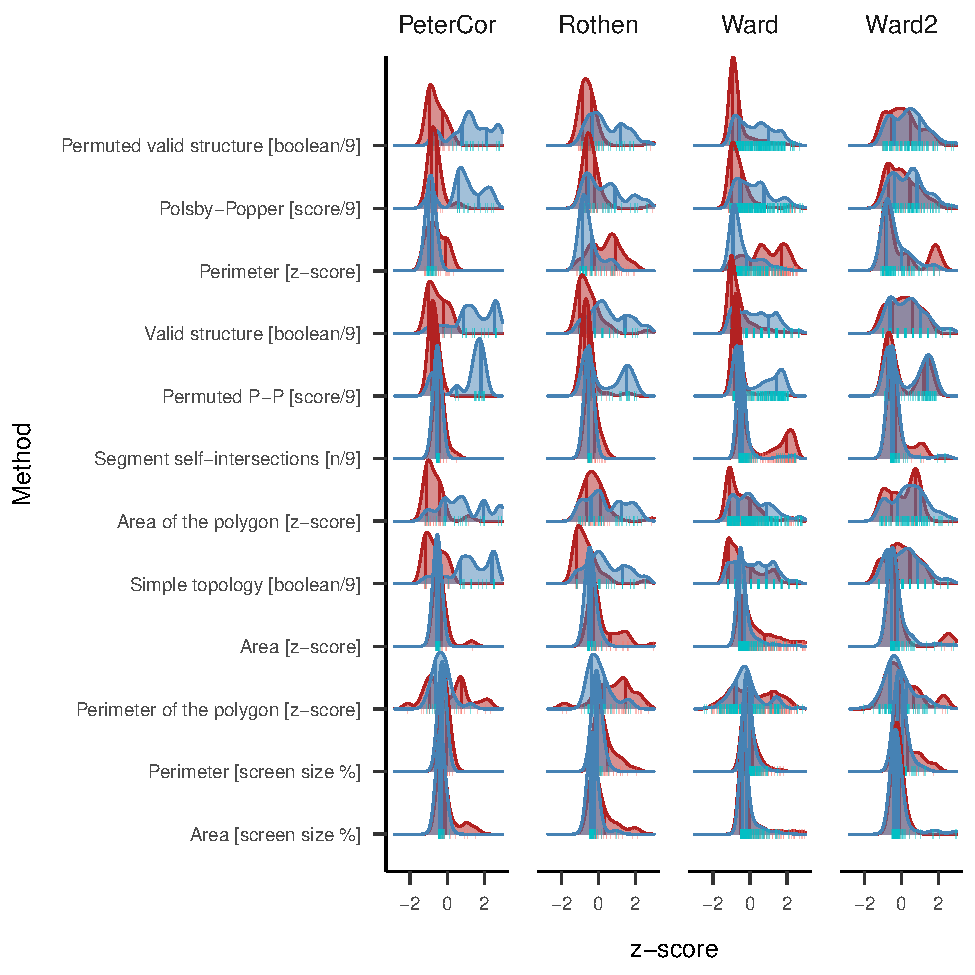
\includegraphics[keepaspectratio]{2.RegisteredReport_MS2_files/figure-pdf/fig-apx08-1.pdf}}

\vspace{-20pt}
\noindent \emph{Note.} Red~= Classified as Synesthetes, Blue = as
controls.

All method's score have been standardized (\emph{z-score}). x axis
treamed between -3 and 3 z-scores. Vertical line indicate respectively
25 and 75 percentiles of each distributions.

\end{figure}

\section{ROC Analysis Sub-sampled data by questionnaire quantiles (20\%
steps)}\label{apx-byquestperc}

We compared the data sampled by the questionnaire score. Based on the
distribution of the questionnaire score, we sampled the 10 \% with the
lowest and 10 \% with the highest scores. Those are then compared with
the 20 and 20 \% and so on until 40 and 40 \%. The rationale of this
procedure is that AUC, sensitivity and specificity should remain stable
across percentiles for a feature to be valid, see
Figure~\ref{fig-myplotapx03}. In other words the ROC should remain
unchanged if we take extreme groups compared to less extreme ones.

\begin{figure}

{\caption{{Lineplots of AUC and DP by questionnaire
percentile}{\label{fig-myplotapx03}}}}

\pandocbounded{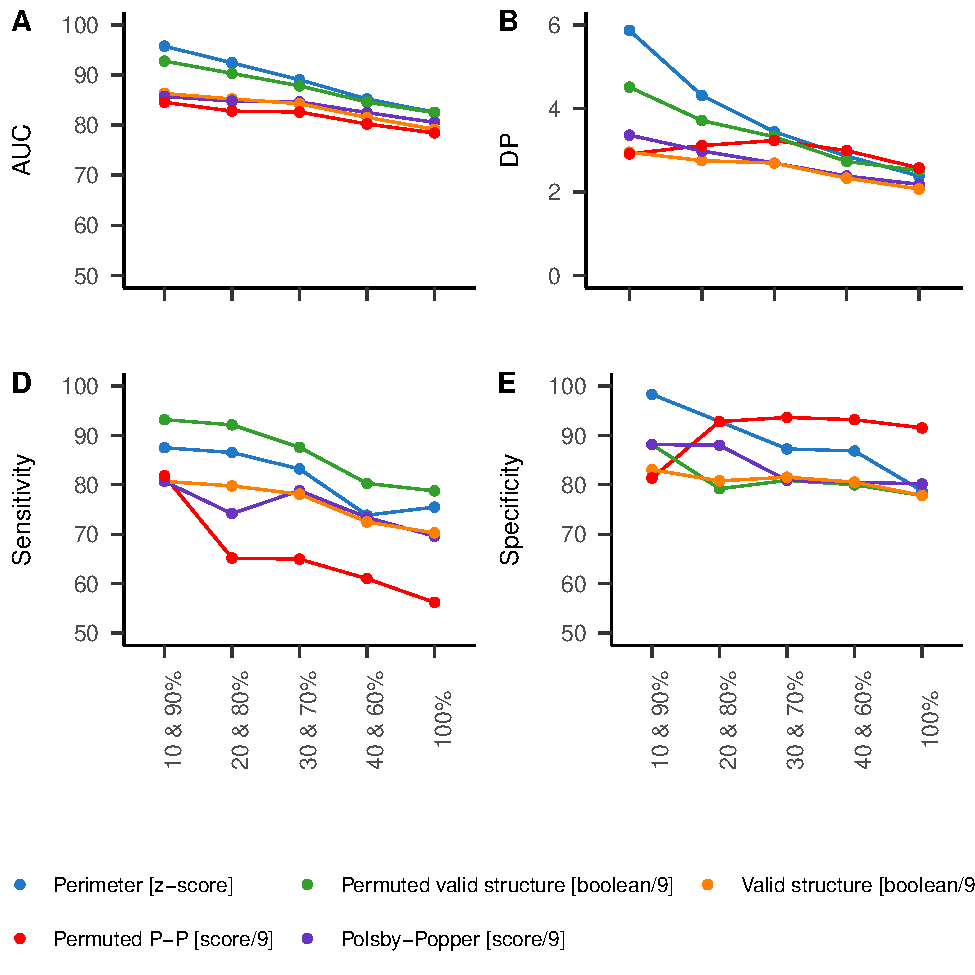
\includegraphics[keepaspectratio]{2.RegisteredReport_MS2_files/figure-pdf/fig-myplotapx03-1.pdf}}

\vspace{-20pt}
\noindent \emph{Note.} Each~point is an increasing percentiles. AUC =
Area Under the Curve. DP = Discrimination Power. Specitficites of some
tests with van Petersen data are 100 \%, so the DP are nor computable
nor interpretable

\end{figure}

\section{Correlation with
self-report}\label{apx-correlation-with-self-report}

The best criterion should also best correlate with SSS self-reported
questionnaire score. Works only with Ward's aggregated data, see
Figure~\ref{fig-myplotapx04}.

\begin{figure}

{\caption{{Correlation with self-reported
questionnaire}{\label{fig-myplotapx04}}}}

\pandocbounded{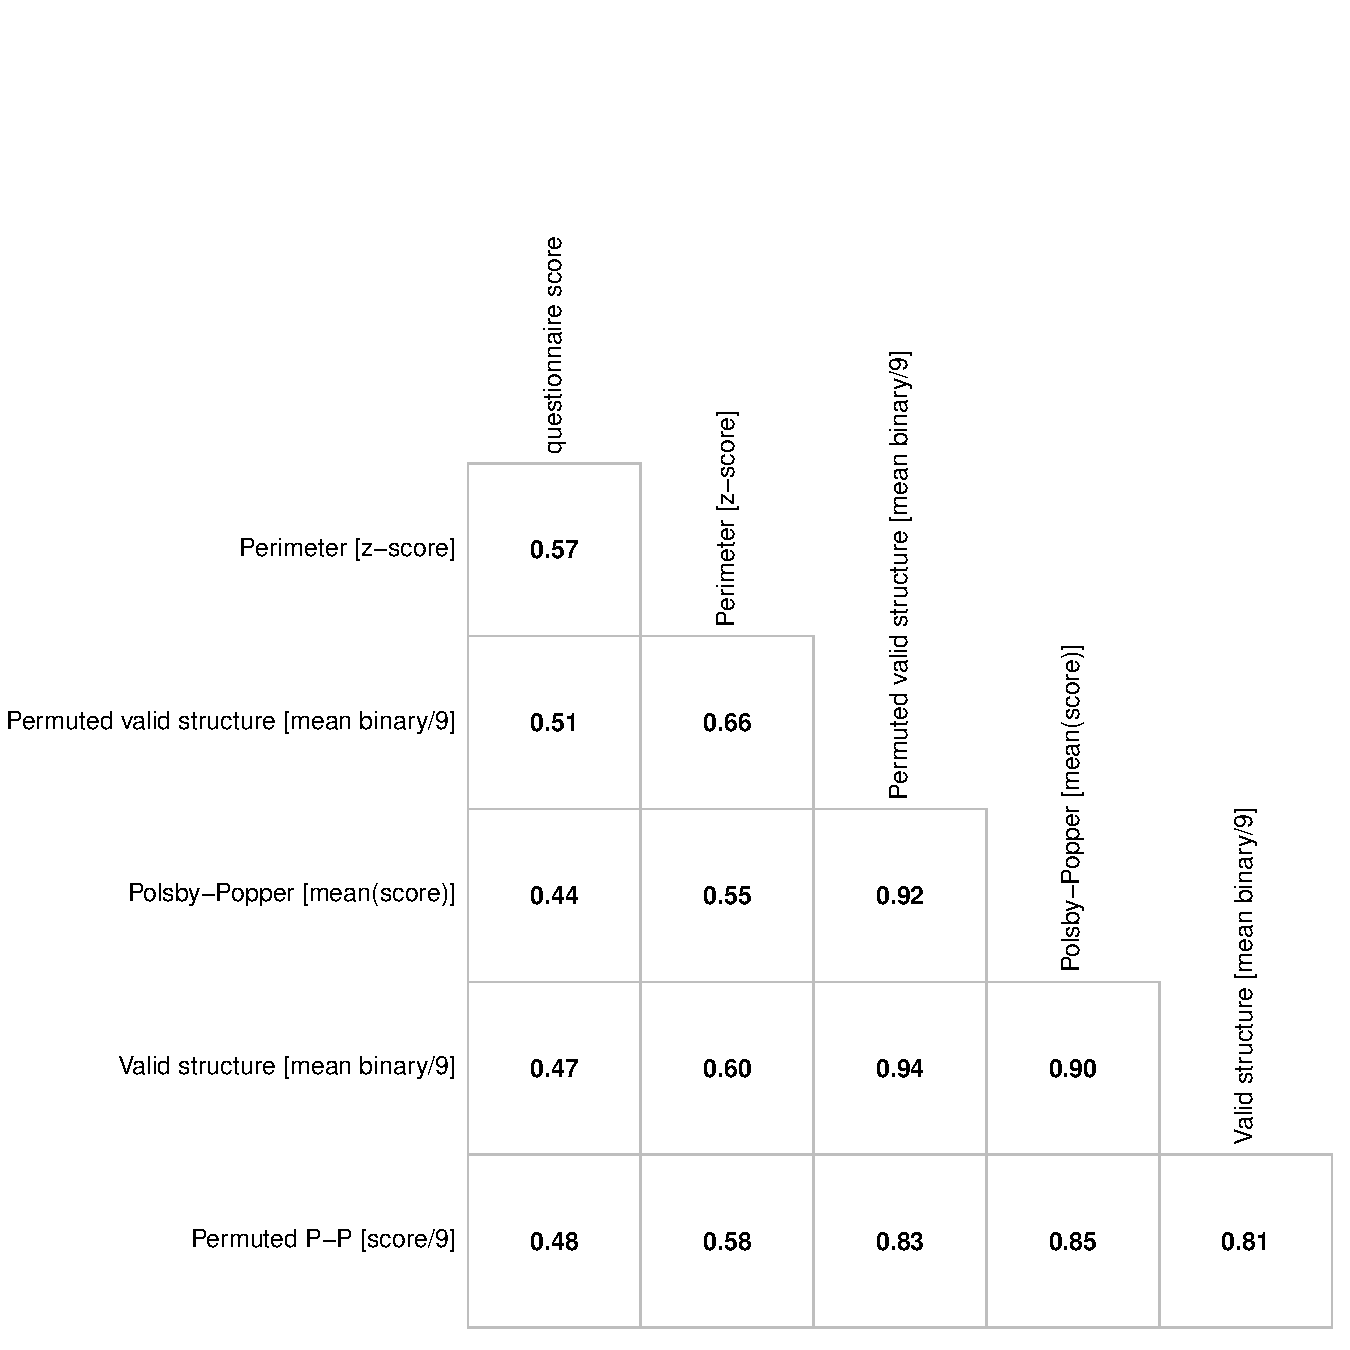
\includegraphics[keepaspectratio]{2.RegisteredReport_MS2_files/figure-pdf/fig-myplotapx04-1.pdf}}

\vspace{-20pt}
\noindent \emph{Note.} Only~data from Ward is included here

\end{figure}

\section{Centred average forms}\label{apx-average-forms}

In this additional analyses we attempted at visualizing the average for
each categories to see whether a pattern could be discerned on a
qualitative level. To avoid negative coordinates, we shifted all the
z-scores from the whole dataset minimum for the x and y coordinates.
Then we anchored to the coordinate 0,0 the stimulus ``1'' for numbers,
``Monday'' for weekdays and ``January'' for months. We then plotted all
the space forms with transparency, see Figure~\ref{fig-myplotapx06}.

Descriptively it is possible to see more circular pattern for months and
horizontal and vertical patterns for numbers. Also the averaged forms
appear to be more clearly defined in the synaesthetes than control.

\begin{figure}

\caption{\label{fig-myplotapx06}Average Centered space forms visualized}

\centering{

\pandocbounded{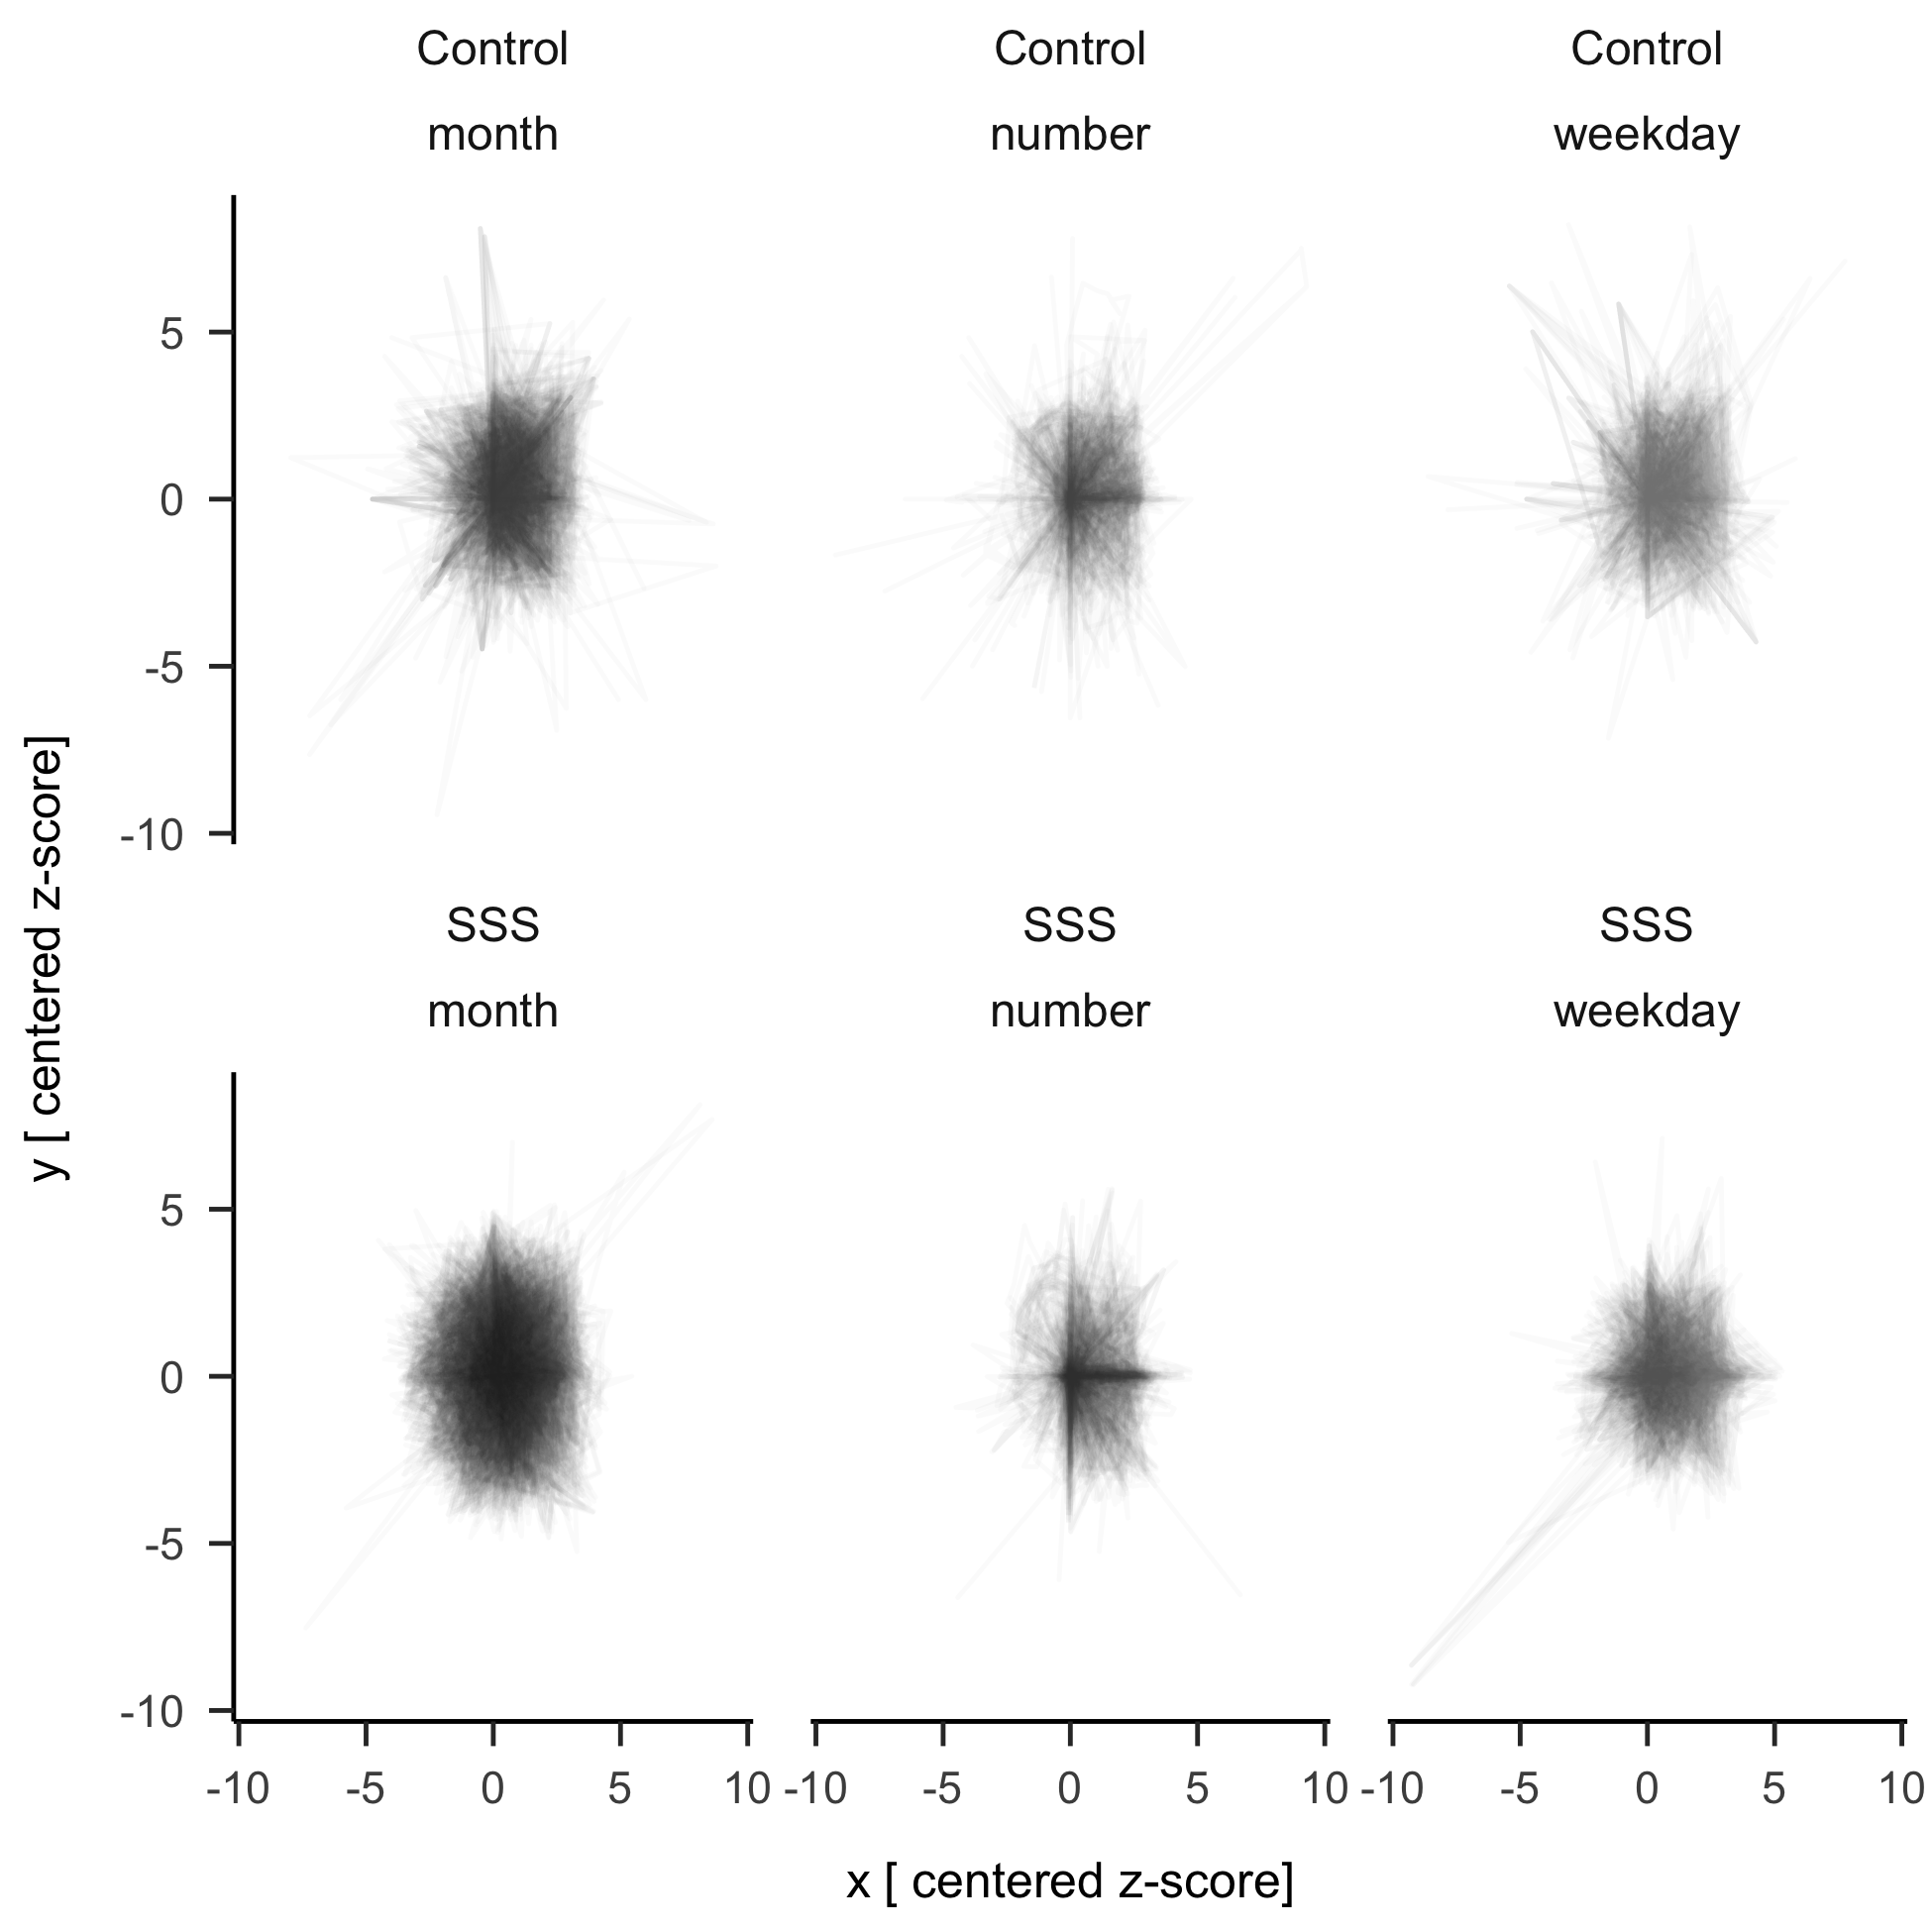
\includegraphics[keepaspectratio]{2.RegisteredReport_MS2_files/figure-pdf/fig-myplotapx06-1.png}}

}

\end{figure}%

\section{Alluvial plot}\label{apx-alluvial}

Are false positives and negatives share some characteristics? To answer
this question qualitatively we identified two group of self-reported SSS
participants who care consistently classified as controls by the five
methods with the highest AUC (i.e.~consistent false negatives), see dark
blue lines in Figure~\ref{fig-myplotapx07}. On the other side we
identified a group of controls who are consistently classified as SSS by
the five methods with the highest AUC, see dark red lines in
Figure~\ref{fig-myplotapx07} .

\begin{figure}

{\caption{{Alluvial plot of test passing}{\label{fig-myplotapx07}}}}

\pandocbounded{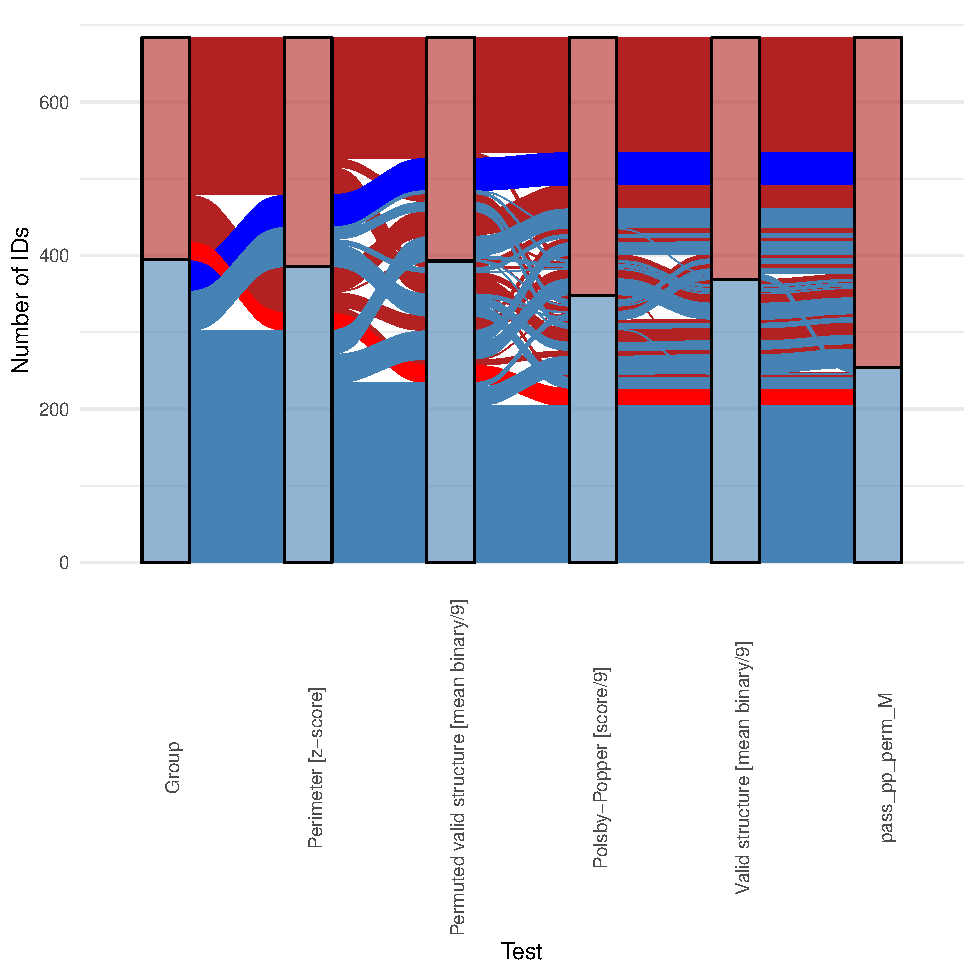
\includegraphics[keepaspectratio]{2.RegisteredReport_MS2_files/figure-pdf/fig-myplotapx07-1.pdf}}

\vspace{-20pt}
\noindent \emph{Note.} Red~= Controls, Blue = Synaesthetes. Highlighted
in blue are Synesthetes who are classified as control by all 5 tests.
Highlighted in red are controls who are classified as synesthetes by all
5 tests.

\end{figure}

On one side 6.12 \% of all participants, that is 42 Synaesthetes where
consistently classified as controls by all five tests, see
Figure~\ref{fig-myplotapx08}. On the other side 3.35 \% of all
participants, 23 controls where consistently classified as SSS by all
five tests, see Figure~\ref{fig-myplotapx09}. Given the different
approaches of each methods, the identified participants might be on one
side non-genuine synesthetes and on the other controls who have SSS but
are either not aware or did not identify it as such.

\begin{figure}

\caption{\label{fig-myplotapx08}Synaesthetes who consistently
\emph{fail} all five tests (blue in the alluvial plot)}

\centering{

\pandocbounded{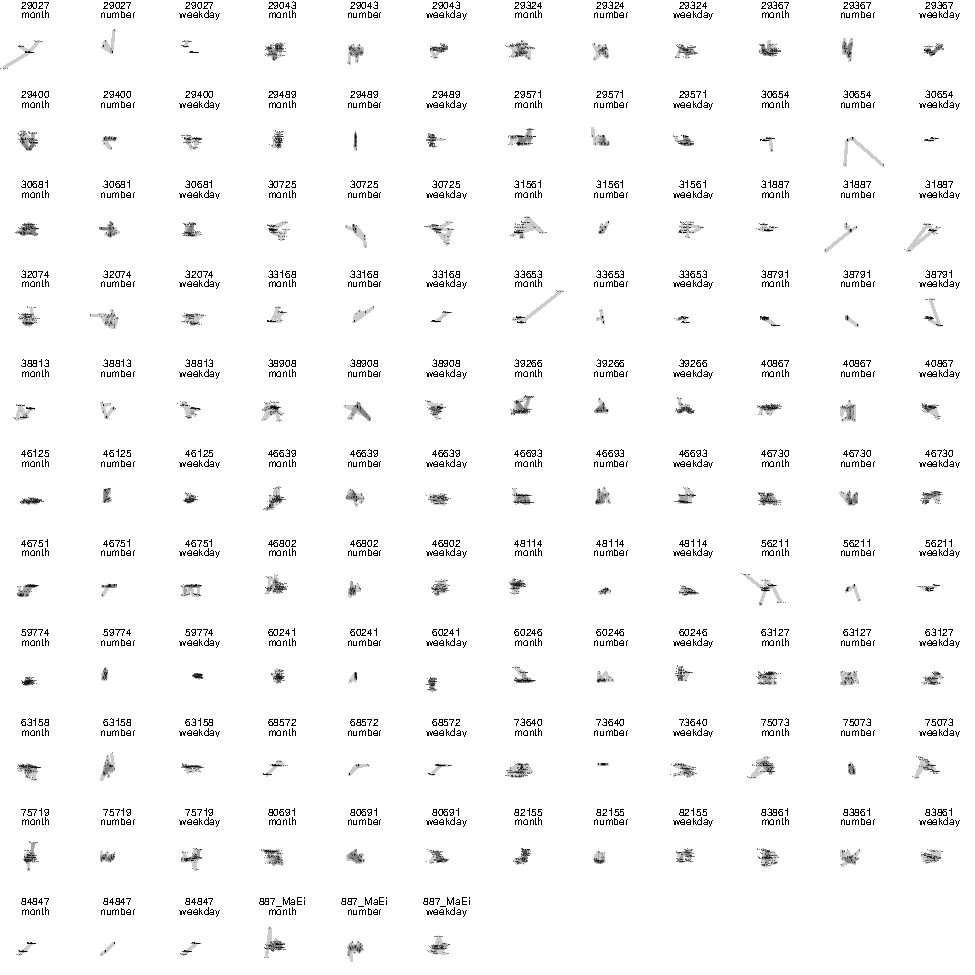
\includegraphics[keepaspectratio]{2.RegisteredReport_MS2_files/figure-pdf/fig-myplotapx08-1.pdf}}

}

\end{figure}%

\begin{figure}

\caption{\label{fig-myplotapx09}Controls who consistently \emph{pass}
all five tests (red in the alluvial plot)}

\centering{

\pandocbounded{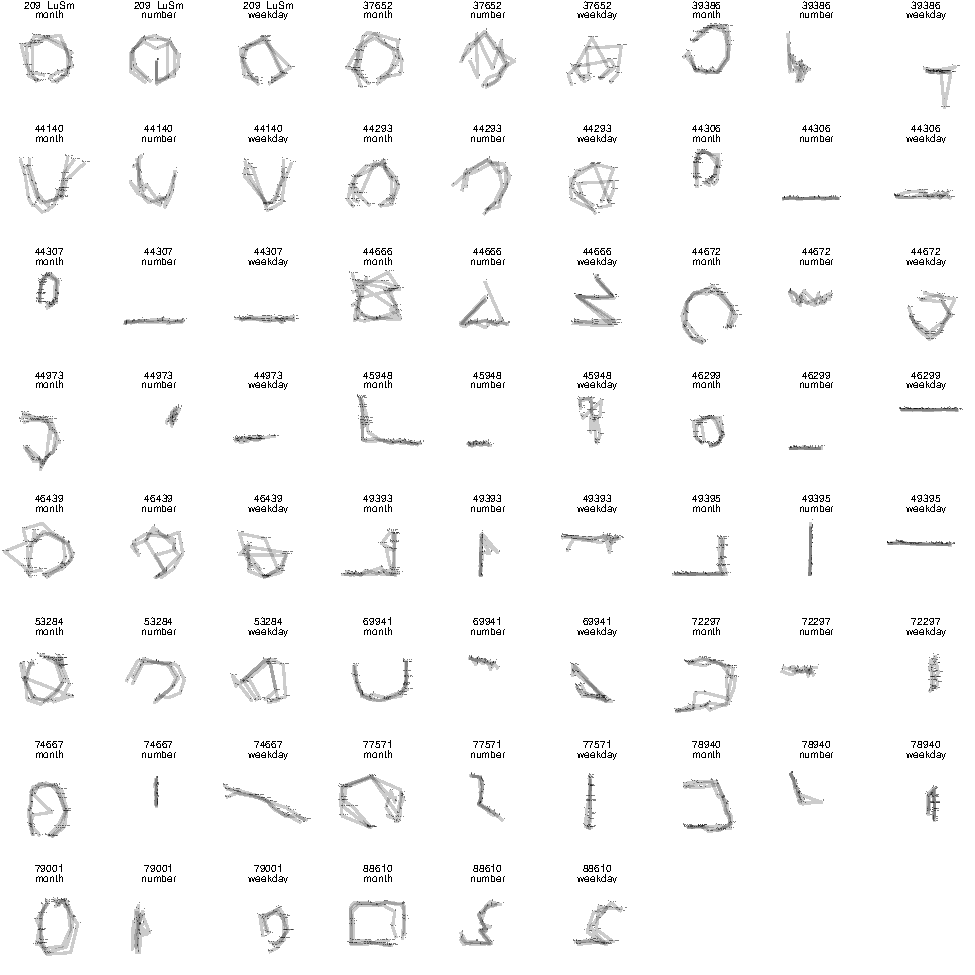
\includegraphics[keepaspectratio]{2.RegisteredReport_MS2_files/figure-pdf/fig-myplotapx09-1.pdf}}

}

\end{figure}%






\end{document}
